\documentclass[11pt]{article}
\usepackage{fontspec}
\setmainfont{NotoSerif-Regular.ttf}[Path=C:/Windows/Fonts/,ItalicFont=NotoSerif-Italic.ttf,BoldFont=NotoSerif-Bold.ttf,BoldItalicFont=NotoSerif-BoldItalic.ttf]
\usepackage[a4paper,margin=22mm]{geometry}
\usepackage{amsmath,amssymb,graphicx,xcolor,hyperref,needspace,tikz}
\usepackage[normalem]{ulem}
\let\MathUnderline\underline
\renewcommand{\underline}[1]{\ifmmode\MathUnderline{#1}\else\uline{#1}\fi}
\hypersetup{unicode=true,colorlinks=true,linkcolor=blue,pdfauthor={}}
\setlength{\parindent}{0pt}
\setlength{\parskip}{.4em}
\setlength{\emergencystretch}{3em}
\raggedright
\newcommand{\SourcePage}[2]{\par\smallskip\phantomsection\label{#1:source-page}{\small\sffamily\color{blue!55!black}#1}\par\smallskip}
\newcommand{\EvidenceBlock}[4]{%
 \par\smallskip\noindent\begin{minipage}{\linewidth}
 \begin{minipage}[t]{.47\linewidth}\vspace{0pt}\centering
 \csname evidence-#1-#2\endcsname\par
 {\scriptsize\SourceCropCaption\ #1}\par
 \end{minipage}\hfill
 \begin{minipage}[t]{.49\linewidth}\vspace{0pt}\raggedright
 {\small\color{orange!65!black}\textbf{#4} #3}\par
 \end{minipage}
 \end{minipage}\par\smallskip}
\newcommand{\Unclear}[3]{\EvidenceBlock{#1}{#2}{#3}{\ReadingCaption}}
\newcommand{\Incomplete}[3]{\EvidenceBlock{#1}{#2}{#3}{\IncompleteCaption}}
\newcommand{\SourceFigure}[3]{\EvidenceBlock{#1}{#2}{#3}{\DiagramCaption}}
\expandafter\def\csname evidence-GELFAND-P000001-module-letter\endcsname{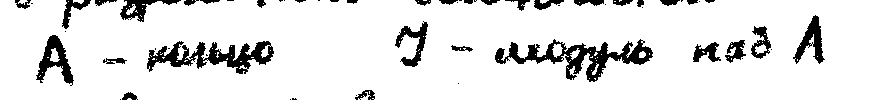
\includegraphics[width=\linewidth]{figures/gelfand-p000001-module-letter-original.png}}
\expandafter\def\csname evidence-GELFAND-P000001-diagram-blowup\endcsname{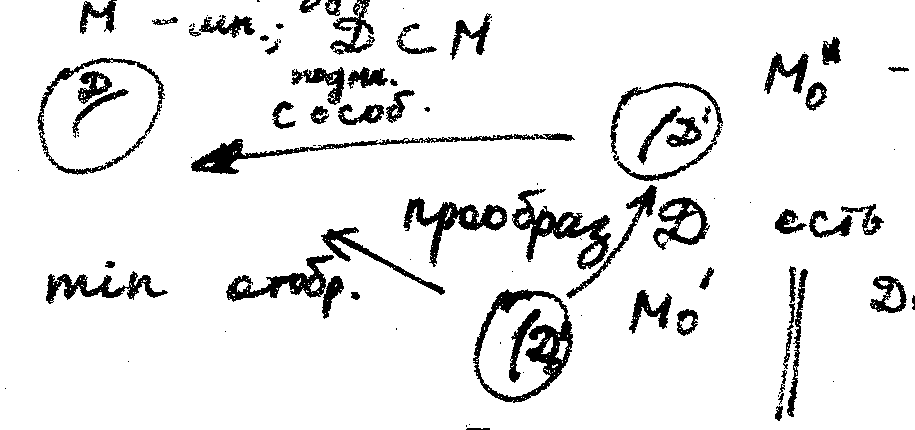
\includegraphics[width=\linewidth]{figures/gelfand-p000001-diagram-blowup-original.png}}
\expandafter\def\csname evidence-GELFAND-P000001-blowup-notation\endcsname{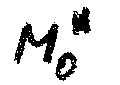
\includegraphics[width=.43\linewidth]{figures/gelfand-p000001-upper-blowup-label-original.png}\hfill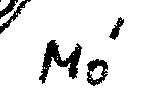
\includegraphics[width=.50\linewidth]{figures/gelfand-p000001-lower-blowup-label-original.png}}
\expandafter\def\csname evidence-GELFAND-P000001-origin-example\endcsname{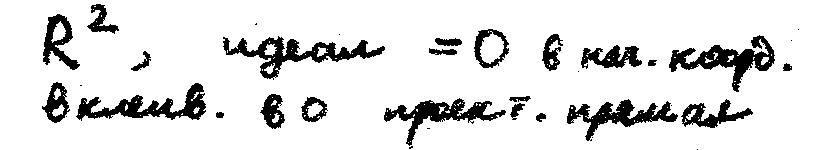
\includegraphics[width=\linewidth]{figures/gelfand-p000001-origin-example-original.png}}
\newcommand{\SourceCropCaption}{Original source details:}\newcommand{\ReadingCaption}{Uncertain reading.}\newcommand{\IncompleteCaption}{Undeciphered passage.}\newcommand{\DiagramCaption}{Diagram and typed description.}
\hypersetup{pdftitle={Gelfand seminar — chapter 1}}

\expandafter\def\csname evidence-GELFAND-P000002-ideal-selection\endcsname{
\includegraphics[width=\linewidth]{figures/gelfand-p000002-ideal-selection-part01-original-r1.png}}
\expandafter\def\csname evidence-GELFAND-P000002-open-set-notation\endcsname{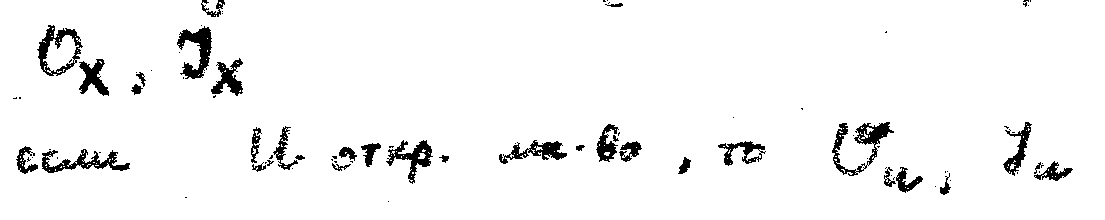
\includegraphics[width=\linewidth]{figures/gelfand-p000002-open-set-notation-part01-original-r2.png}}
\expandafter\def\csname evidence-GELFAND-P000002-fractions-sentence\endcsname{
\includegraphics[width=\linewidth]{figures/gelfand-p000002-fractions-sentence-part01-original-r1.png}\par\smallskip
\includegraphics[width=\linewidth]{figures/gelfand-p000002-fractions-sentence-part02-original-r1.png}\par\smallskip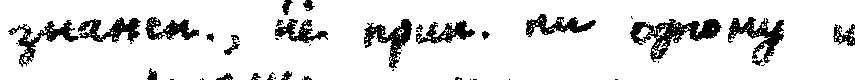
\includegraphics[width=\linewidth]{figures/gelfand-p000002-fractions-sentence-part03-original-r1.png}\par\smallskip
\includegraphics[width=\linewidth]{figures/gelfand-p000002-fractions-sentence-part04-original-r1.png}}
\expandafter\def\csname evidence-GELFAND-P000002-margin-grothendieck\endcsname{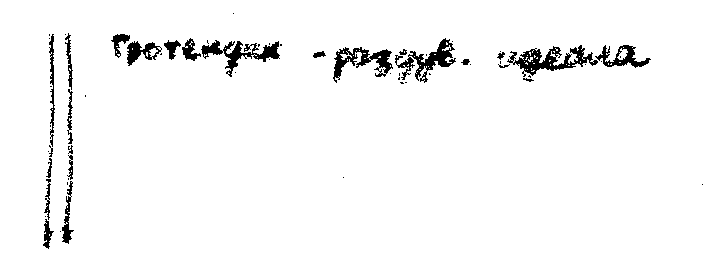
\includegraphics[width=\linewidth]{figures/gelfand-p000002-margin-grothendieck-part01-original-r1.png}}
\expandafter\def\csname evidence-GELFAND-P000002-quadratic-coefficients\endcsname{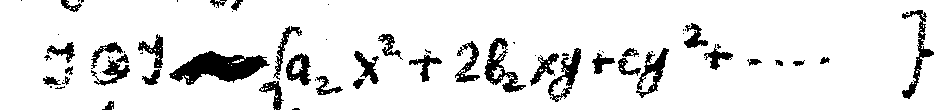
\includegraphics[width=\linewidth]{figures/gelfand-p000002-quadratic-coefficients-part01-original-r1.png}}
\expandafter\def\csname evidence-GELFAND-P000002-last-sign\endcsname{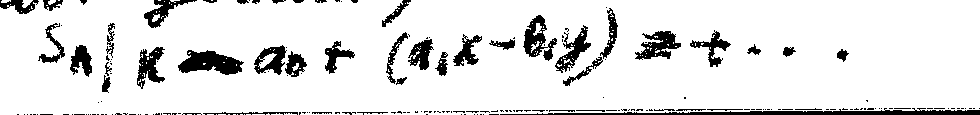
\includegraphics[width=\linewidth]{figures/gelfand-p000002-last-sign-part01-original-r1.png}}
\expandafter\def\csname evidence-GELFAND-P000003-directions\endcsname{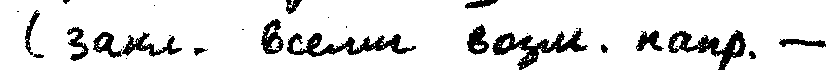
\includegraphics[width=\linewidth]{figures/gelfand-p000003-directions-part01-original-r1.png}\par\smallskip
\includegraphics[width=\linewidth]{figures/gelfand-p000003-directions-part02-original-r1.png}}
\expandafter\def\csname evidence-GELFAND-P000003-cross-cancellation\endcsname{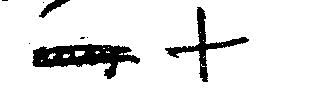
\includegraphics[width=\linewidth]{figures/gelfand-p000003-cross-cancellation-part01-original-r1.png}}
\expandafter\def\csname evidence-GELFAND-P000003-ising-cancellation\endcsname{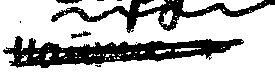
\includegraphics[width=\linewidth]{figures/gelfand-p000003-ising-cancellation-part01-original-r1.png}}
\expandafter\def\csname evidence-GELFAND-P000003-configuration-letter\endcsname{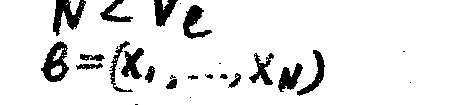
\includegraphics[width=\linewidth]{figures/gelfand-p000003-configuration-letter-part01-original-r2.png}}
\expandafter\def\csname evidence-GELFAND-P000003-energy-cancellation\endcsname{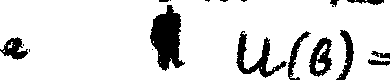
\includegraphics[width=\linewidth]{figures/gelfand-p000003-energy-cancellation-part01-original-r1.png}}
\expandafter\def\csname evidence-GELFAND-P000003-energy-case\endcsname{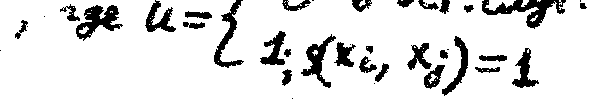
\includegraphics[width=\linewidth]{figures/gelfand-p000003-energy-case-part01-original-r2.png}\par\smallskip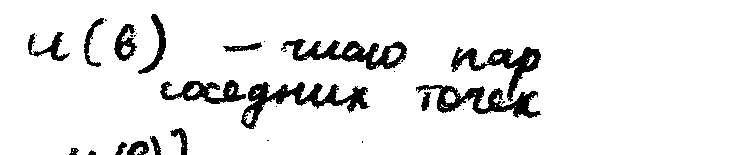
\includegraphics[width=\linewidth]{figures/gelfand-p000003-energy-case-part02-original-r3.png}}
\expandafter\def\csname evidence-GELFAND-P000003-partition-domain\endcsname{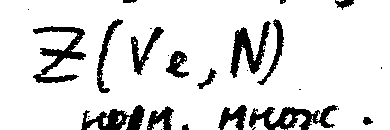
\includegraphics[width=\linewidth]{figures/gelfand-p000003-partition-domain-part01-original-r1.png}\par\smallskip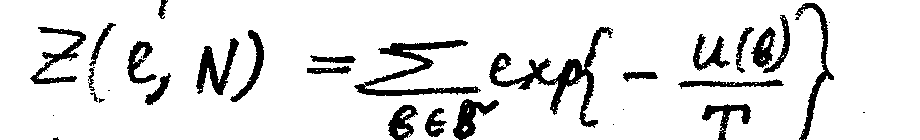
\includegraphics[width=\linewidth]{figures/gelfand-p000003-partition-domain-part02-original-r1.png}}
\expandafter\def\csname evidence-GELFAND-P000003-attraction-note\endcsname{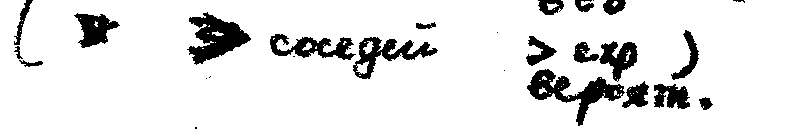
\includegraphics[width=\linewidth]{figures/gelfand-p000003-attraction-note-part01-original-r1.png}}
\expandafter\def\csname evidence-GELFAND-P000003-density-cancellation\endcsname{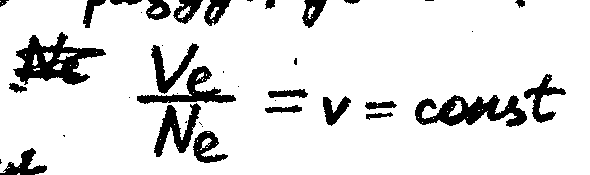
\includegraphics[width=\linewidth]{figures/gelfand-p000003-density-cancellation-part01-original-r1.png}}

\expandafter\def\csname evidence-GELFAND-P000004-pressure-letter\endcsname{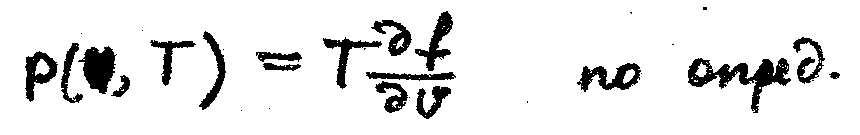
\includegraphics[width=\linewidth]{figures/gelfand-p000004-pressure-letter-part01-original-r1.png}}
\expandafter\def\csname evidence-GELFAND-P000004-diagram-phase-point\endcsname{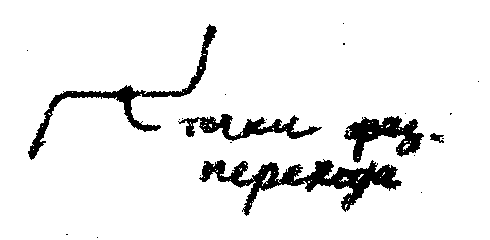
\includegraphics[width=\linewidth]{figures/gelfand-p000004-diagram-phase-point-part01-original-r2.png}}
\expandafter\def\csname evidence-GELFAND-P000004-diagram-cancelled-graph\endcsname{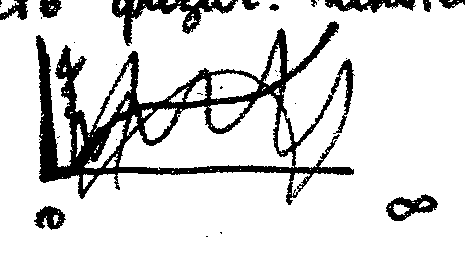
\includegraphics[width=\linewidth]{figures/gelfand-p000004-diagram-cancelled-graph-part01-original-r1.png}}
\expandafter\def\csname evidence-GELFAND-P000004-diagram-onsager\endcsname{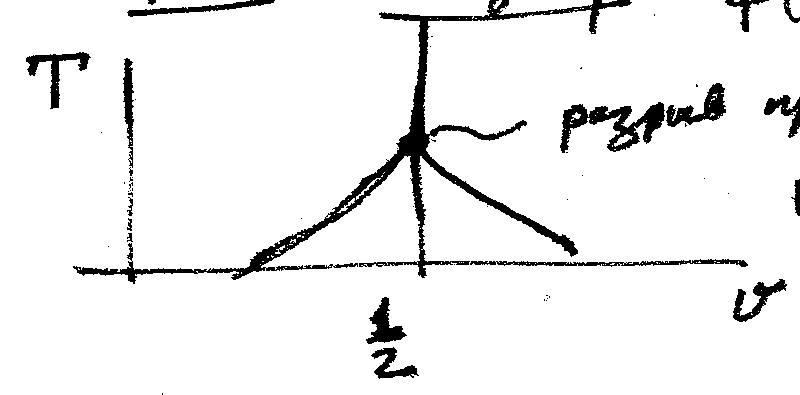
\includegraphics[width=\linewidth]{figures/gelfand-p000004-diagram-onsager-part01-original-r1.png}}
\expandafter\def\csname evidence-GELFAND-P000004-kac-helfand-note\endcsname{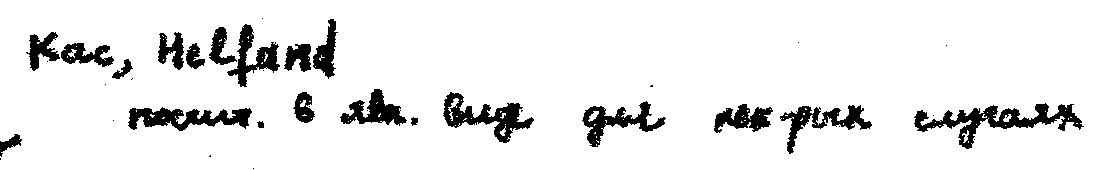
\includegraphics[width=\linewidth]{figures/gelfand-p000004-kac-helfand-note-part01-original-r1.png}}
\expandafter\def\csname evidence-GELFAND-P000004-diagram-subcube\endcsname{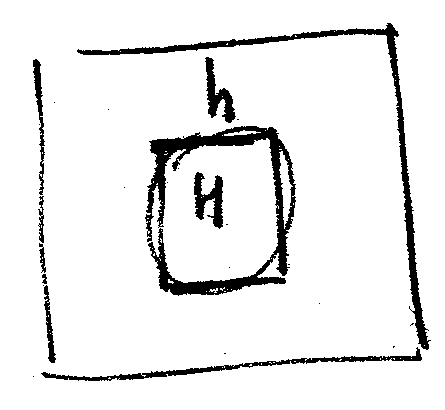
\includegraphics[width=\linewidth]{figures/gelfand-p000004-diagram-subcube-part01-original-r1.png}}
\expandafter\def\csname evidence-GELFAND-P000004-probability-bar\endcsname{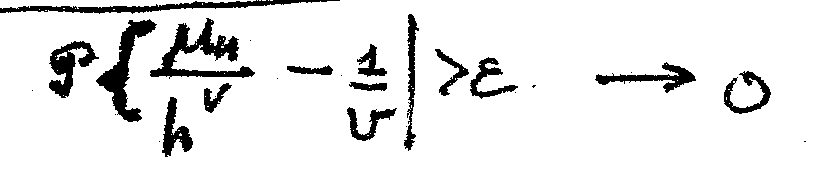
\includegraphics[width=\linewidth]{figures/gelfand-p000004-probability-bar-part01-original-r1.png}}
\expandafter\def\csname evidence-GELFAND-P000004-bottom-mark\endcsname{
\includegraphics[width=\linewidth]{figures/gelfand-p000004-bottom-mark-part01-original-r1.png}}
\expandafter\def\csname evidence-GELFAND-P000004-margin-left\endcsname{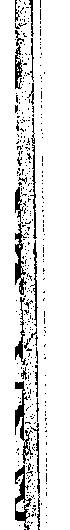
\includegraphics[height=60mm]{figures/gelfand-p000004-margin-left-part01-original-r1.png}\hspace{2mm}
\includegraphics[height=60mm]{figures/gelfand-p000004-margin-left-part02-original-r1.png}\hspace{2mm}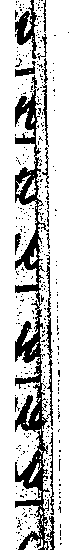
\includegraphics[height=60mm]{figures/gelfand-p000004-margin-left-part03-original-r1.png}\hspace{2mm}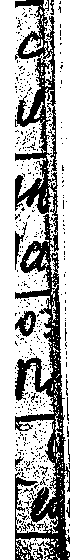
\includegraphics[height=60mm]{figures/gelfand-p000004-margin-left-part04-original-r1.png}}
\expandafter\def\csname evidence-GELFAND-P000005-exponential-rate\endcsname{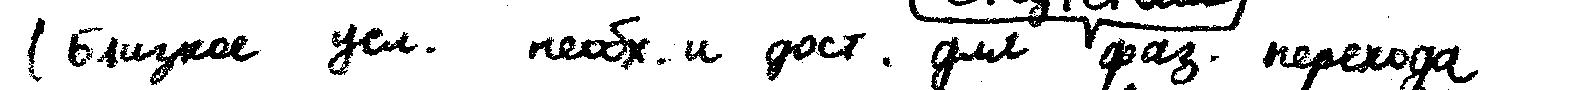
\includegraphics[width=\linewidth]{figures/gelfand-p000005-exponential-rate-part01-original-r1.png}\par\smallskip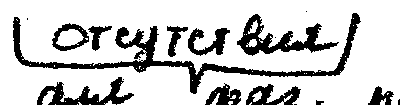
\includegraphics[width=\linewidth]{figures/gelfand-p000005-exponential-rate-part02-original-r1.png}\par\smallskip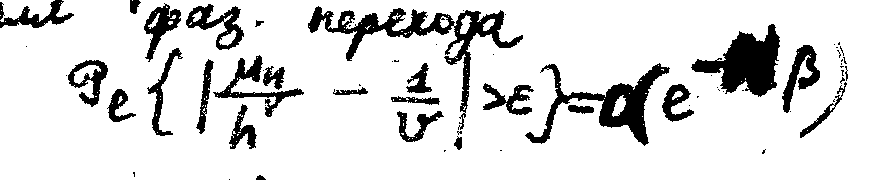
\includegraphics[width=\linewidth]{figures/gelfand-p000005-exponential-rate-part03-original-r2.png}}
\expandafter\def\csname evidence-GELFAND-P000005-complement-label\endcsname{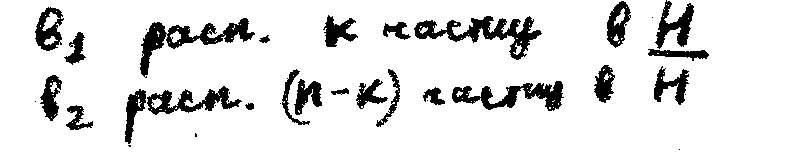
\includegraphics[width=\linewidth]{figures/gelfand-p000005-complement-label-part01-original-r1.png}}
\expandafter\def\csname evidence-GELFAND-P000005-boundary-exponent\endcsname{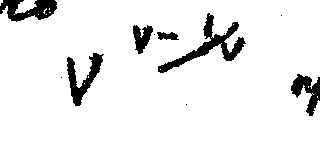
\includegraphics[width=\linewidth]{figures/gelfand-p000005-boundary-exponent-part01-original-r1.png}\par\smallskip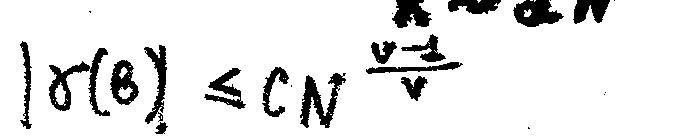
\includegraphics[width=\linewidth]{figures/gelfand-p000005-boundary-exponent-part02-original-r1.png}}
\expandafter\def\csname evidence-GELFAND-P000005-theta-factor\endcsname{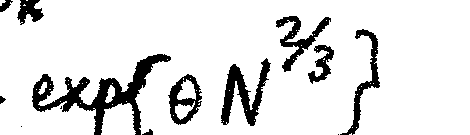
\includegraphics[width=\linewidth]{figures/gelfand-p000005-theta-factor-part01-original-r1.png}\par\smallskip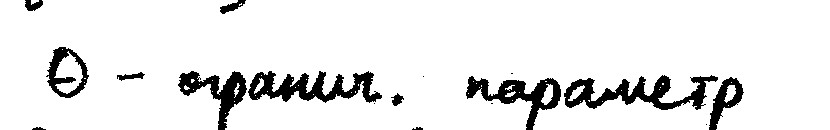
\includegraphics[width=\linewidth]{figures/gelfand-p000005-theta-factor-part02-original-r1.png}\par\smallskip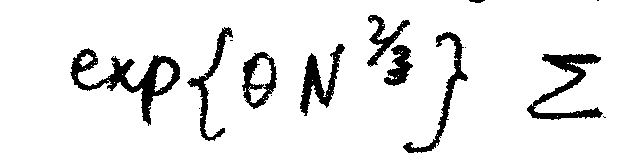
\includegraphics[width=\linewidth]{figures/gelfand-p000005-theta-factor-part03-original-r1.png}}
\expandafter\def\csname evidence-GELFAND-P000005-physical-meaning-heading\endcsname{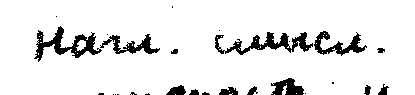
\includegraphics[width=\linewidth]{figures/gelfand-p000005-physical-meaning-heading-part01-original-r1.png}}
\expandafter\def\csname evidence-GELFAND-P000004-diagram-pressure-plateau\endcsname{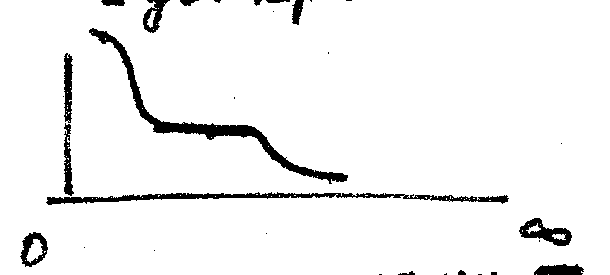
\includegraphics[width=\linewidth]{figures/gelfand-p000004-diagram-pressure-plateau-original-r1.png}}
\newcommand{\PhaseWords}{points of phase\\transition}

\expandafter\def\csname evidence-GELFAND-P000006-subcube-power\endcsname{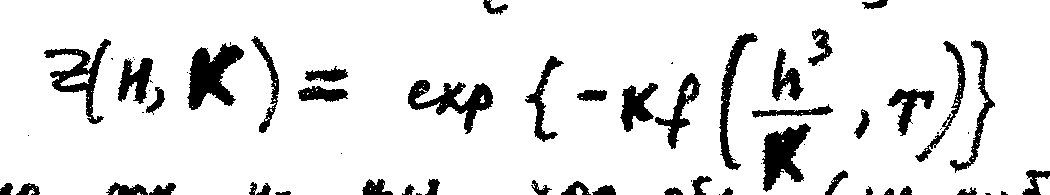
\includegraphics[width=\linewidth]{figures/gelfand-p000006-subcube-power-part01-original-r1.png}\par\smallskip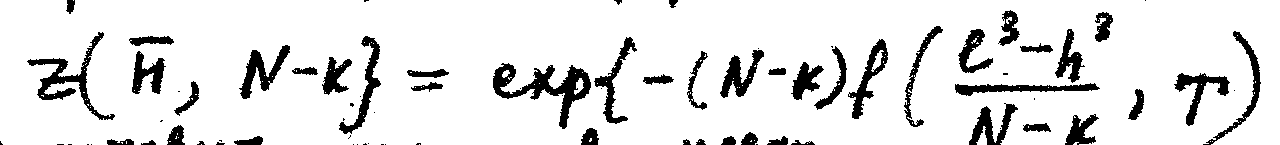
\includegraphics[width=\linewidth]{figures/gelfand-p000006-subcube-power-part02-original-r1.png}}
\expandafter\def\csname evidence-GELFAND-P000006-limit-notation\endcsname{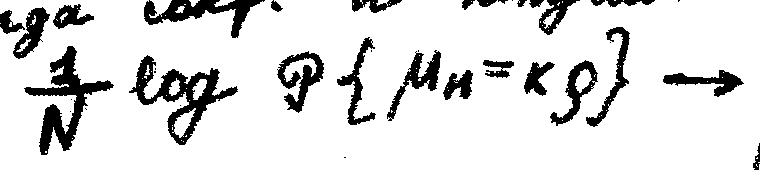
\includegraphics[width=\linewidth]{figures/gelfand-p000006-limit-notation-part01-original-r1.png}\par\smallskip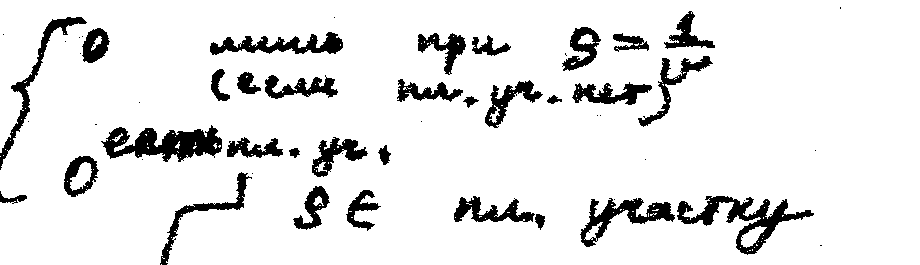
\includegraphics[width=\linewidth]{figures/gelfand-p000006-limit-notation-part02-original-r1.png}}
\expandafter\def\csname evidence-GELFAND-P000006-diagram-limit-step\endcsname{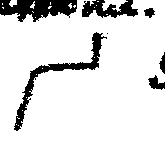
\includegraphics[width=\linewidth]{figures/gelfand-p000006-diagram-limit-step-part01-original-r1.png}}
\expandafter\def\csname evidence-GELFAND-P000006-diagram-cell-clusters\endcsname{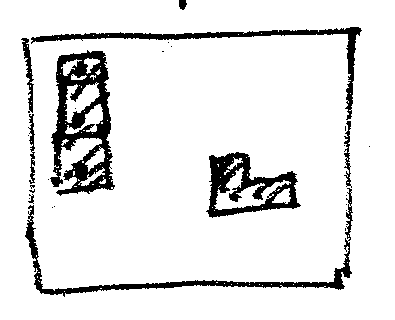
\includegraphics[width=\linewidth]{figures/gelfand-p000006-diagram-cell-clusters-part01-original-r1.png}}
\expandafter\def\csname evidence-GELFAND-P000006-gamma-prime\endcsname{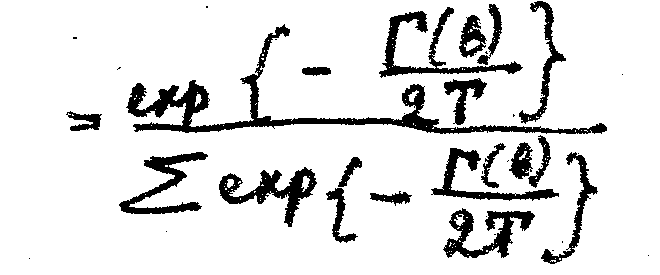
\includegraphics[width=\linewidth]{figures/gelfand-p000006-gamma-prime-part01-original-r1.png}}
\expandafter\def\csname evidence-GELFAND-P000006-energy-bound\endcsname{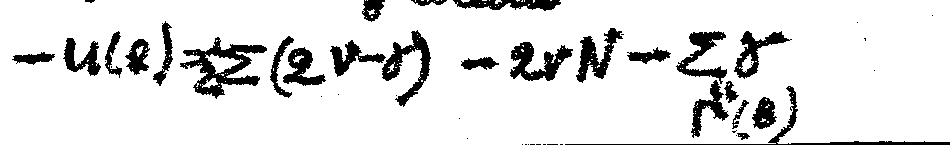
\includegraphics[width=\linewidth]{figures/gelfand-p000006-energy-bound-part01-original-r1.png}}
\expandafter\def\csname evidence-GELFAND-P000007-diagram-small-clusters\endcsname{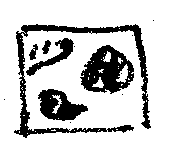
\includegraphics[width=\linewidth]{figures/gelfand-p000007-diagram-small-clusters-part01-original-r1.png}}
\expandafter\def\csname evidence-GELFAND-P000007-diagram-cycles\endcsname{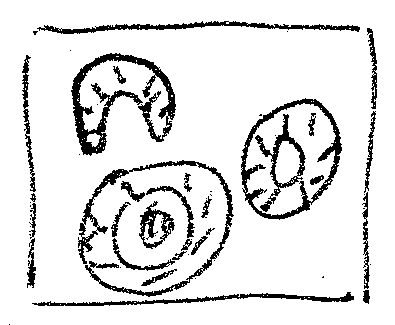
\includegraphics[width=\linewidth]{figures/gelfand-p000007-diagram-cycles-part01-original-r1.png}}
\expandafter\def\csname evidence-GELFAND-P000007-special-arrangement-count\endcsname{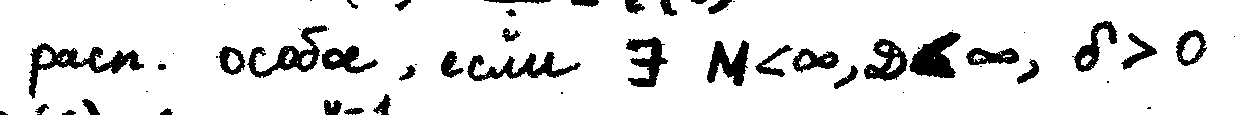
\includegraphics[width=\linewidth]{figures/gelfand-p000007-special-arrangement-count-part01-original-r1.png}}
\expandafter\def\csname evidence-GELFAND-P000007-large-cycles-power\endcsname{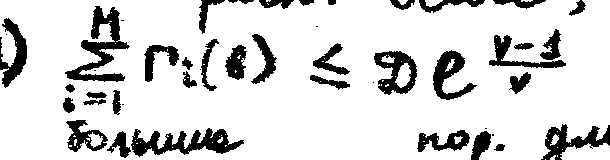
\includegraphics[width=\linewidth]{figures/gelfand-p000007-large-cycles-power-part01-original-r1.png}}
\expandafter\def\csname evidence-GELFAND-P000007-small-cycles-sum\endcsname{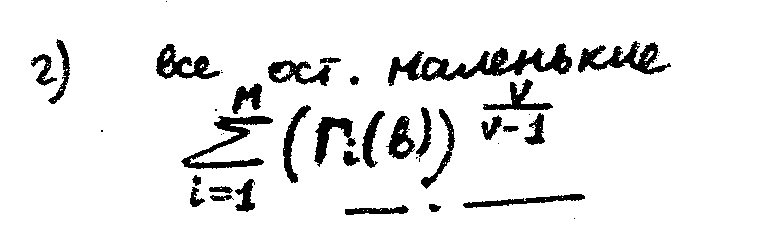
\includegraphics[width=\linewidth]{figures/gelfand-p000007-small-cycles-sum-part01-original-r1.png}}
\expandafter\def\csname evidence-GELFAND-P000007-field-margin\endcsname{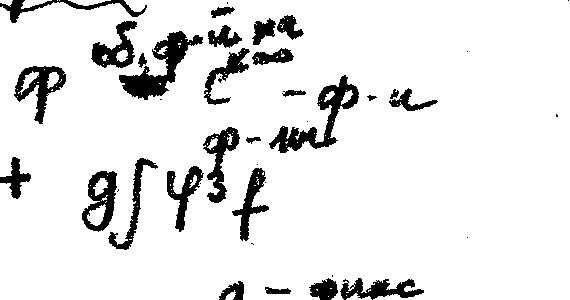
\includegraphics[width=\linewidth]{figures/gelfand-p000007-field-margin-part01-original-r1.png}}
\expandafter\def\csname evidence-GELFAND-P000007-evaluation-target\endcsname{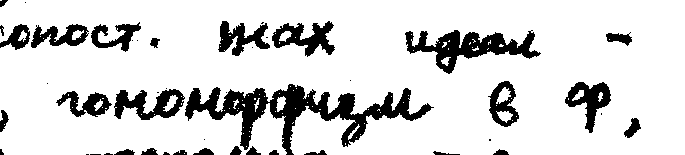
\includegraphics[width=\linewidth]{figures/gelfand-p000007-evaluation-target-part01-original-r1.png}}
\expandafter\def\csname evidence-GELFAND-P000008-linear-oscillation\endcsname{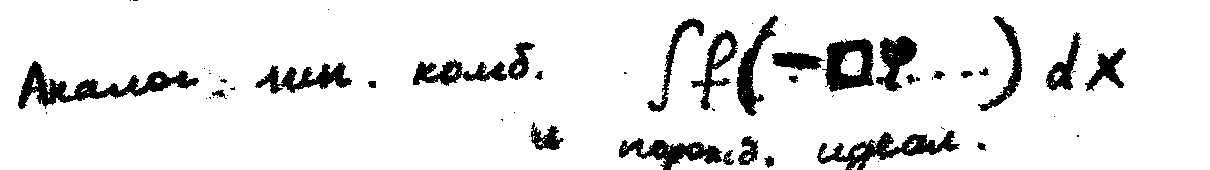
\includegraphics[width=\linewidth]{figures/gelfand-p000008-linear-oscillation-part01-original-r1.png}}
\expandafter\def\csname evidence-GELFAND-P000008-name-van-hove\endcsname{
\includegraphics[width=\linewidth]{figures/gelfand-p000008-name-van-hove-part01-original-r1.png}}
\expandafter\def\csname evidence-GELFAND-P000008-temperature-relation\endcsname{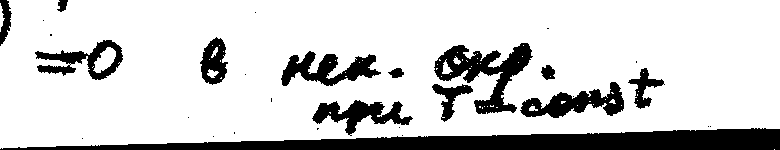
\includegraphics[width=\linewidth]{figures/gelfand-p000008-temperature-relation-part01-original-r1.png}}
\expandafter\def\csname evidence-GELFAND-P000008-margin-left\endcsname{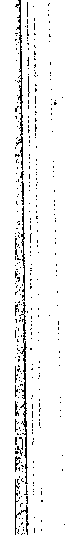
\includegraphics[height=60mm]{figures/gelfand-p000008-margin-left-part01-original-r1.png}\hspace{2mm}
\includegraphics[height=60mm]{figures/gelfand-p000008-margin-left-part02-original-r1.png}\hspace{2mm}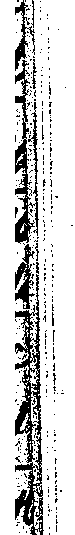
\includegraphics[height=60mm]{figures/gelfand-p000008-margin-left-part03-original-r1.png}\hspace{2mm}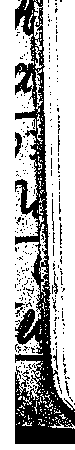
\includegraphics[height=60mm]{figures/gelfand-p000008-margin-left-part04-original-r1.png}}
\expandafter\def\csname evidence-GELFAND-P000009-sphere-constant\endcsname{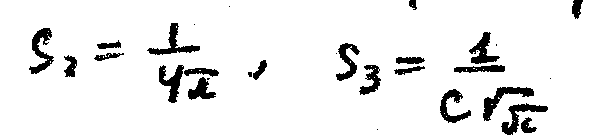
\includegraphics[width=\linewidth]{figures/gelfand-p000009-sphere-constant-part01-original-r1.png}}
\expandafter\def\csname evidence-GELFAND-P000009-probability-brace\endcsname{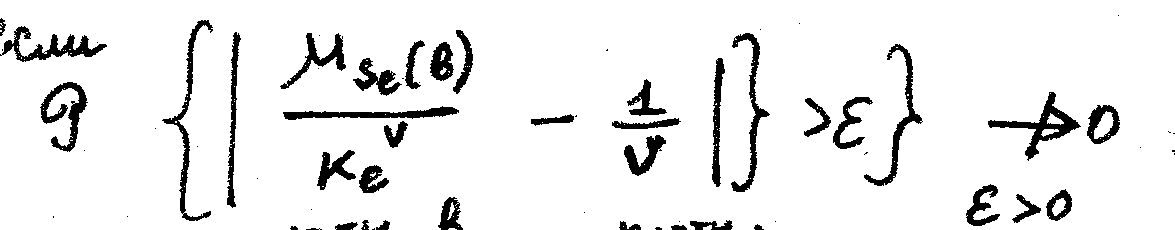
\includegraphics[width=\linewidth]{figures/gelfand-p000009-probability-brace-part01-original-r1.png}}
\expandafter\def\csname evidence-GELFAND-P000010-diagram-nested-cycles\endcsname{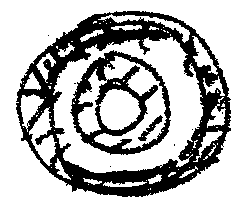
\includegraphics[width=\linewidth]{figures/gelfand-p000010-diagram-nested-cycles-part01-original-r1.png}}
\expandafter\def\csname evidence-GELFAND-P000010-diagram-phase-mixture\endcsname{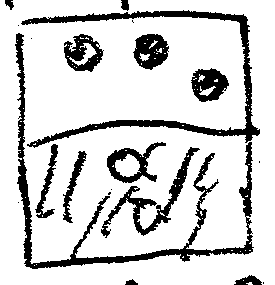
\includegraphics[width=\linewidth]{figures/gelfand-p000010-diagram-phase-mixture-part01-original-r1.png}}
\expandafter\def\csname evidence-GELFAND-P000007-ideal-signature\endcsname{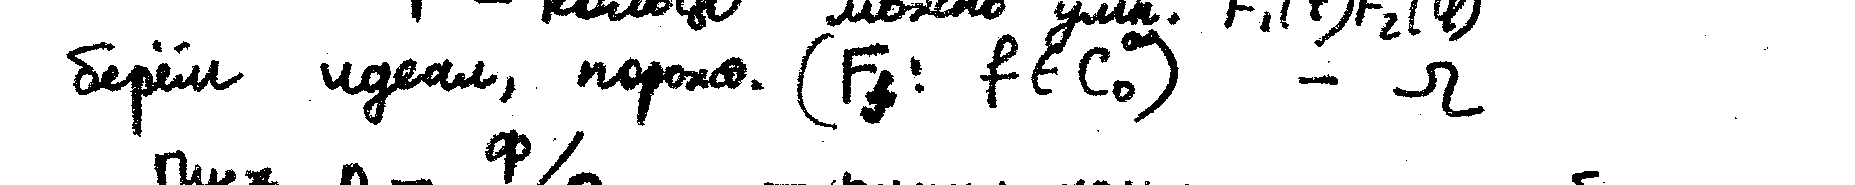
\includegraphics[width=\linewidth]{figures/gelfand-p000007-ideal-signature-part01-original-r2.png}}
\expandafter\def\csname evidence-GELFAND-P000008-algebra-ring-letter\endcsname{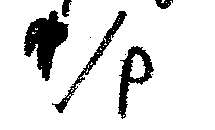
\includegraphics[width=\linewidth]{figures/gelfand-p000008-algebra-ring-letter-part01-original-r2.png}\par\smallskip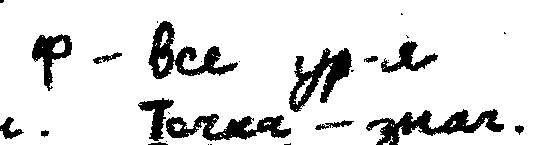
\includegraphics[width=\linewidth]{figures/gelfand-p000008-algebra-ring-letter-part02-original-r2.png}}
\expandafter\def\csname evidence-GELFAND-P000009-q-formula\endcsname{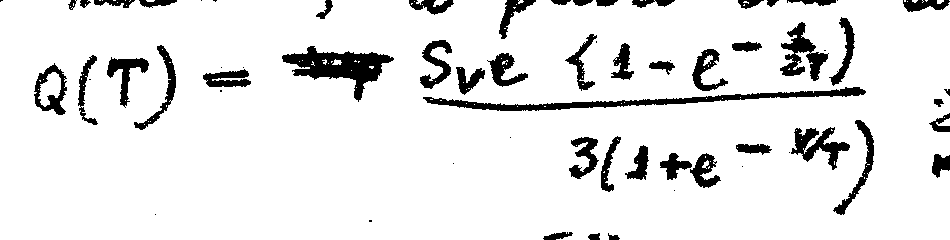
\includegraphics[width=\linewidth]{figures/gelfand-p000009-q-formula-part01-original-r2.png}\par\smallskip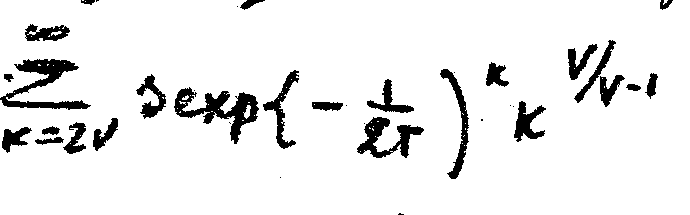
\includegraphics[width=\linewidth]{figures/gelfand-p000009-q-formula-part02-original-r2.png}}
\expandafter\def\csname evidence-GELFAND-P000009-finite-parameter\endcsname{
\includegraphics[width=\linewidth]{figures/gelfand-p000009-finite-parameter-part01-original-r2.png}}
\expandafter\def\csname evidence-GELFAND-P000010-small-cycles-sign\endcsname{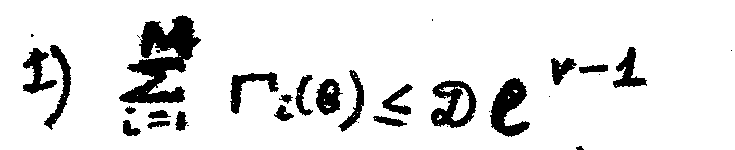
\includegraphics[width=\linewidth]{figures/gelfand-p000010-small-cycles-sign-part01-original-r2.png}\par\smallskip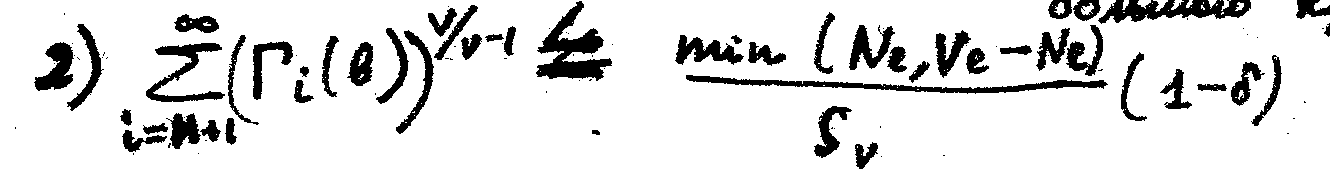
\includegraphics[width=\linewidth]{figures/gelfand-p000010-small-cycles-sign-part02-original-r2.png}}
\expandafter\def\csname evidence-GELFAND-P000010-small-volume-cancellation\endcsname{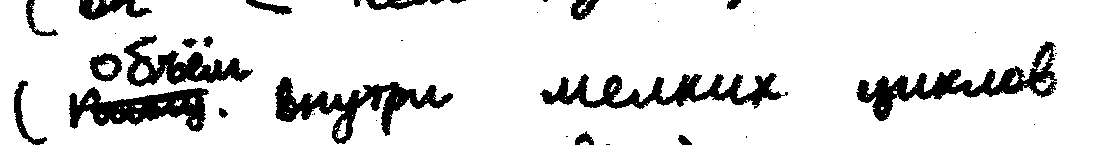
\includegraphics[width=\linewidth]{figures/gelfand-p000010-small-volume-cancellation-part01-original-r2.png}\par\smallskip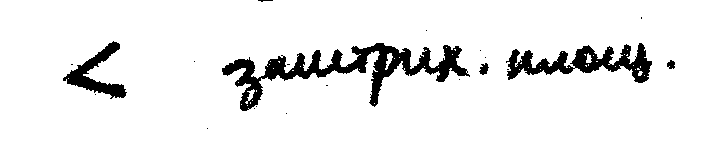
\includegraphics[width=\linewidth]{figures/gelfand-p000010-small-volume-cancellation-part02-original-r2.png}\par\smallskip
\includegraphics[width=\linewidth]{figures/gelfand-p000010-small-volume-cancellation-part03-original-r2.png}}
\expandafter\def\csname evidence-GELFAND-P000010-theorem-condition\endcsname{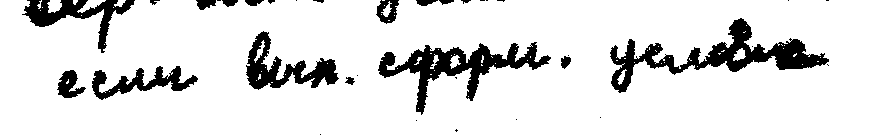
\includegraphics[width=\linewidth]{figures/gelfand-p000010-theorem-condition-part01-original-r2.png}}
\expandafter\def\csname evidence-GELFAND-P000010-diagram-grid\endcsname{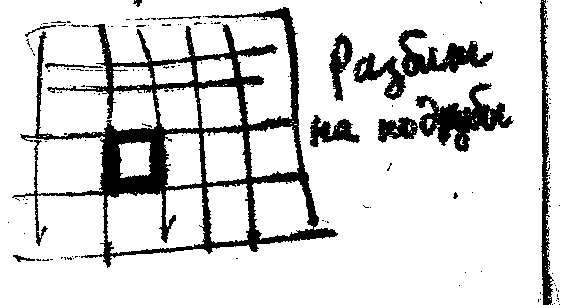
\includegraphics[width=\linewidth]{figures/gelfand-p000010-diagram-grid-part01-original-r2.png}}
\expandafter\def\csname evidence-GELFAND-P000010-last-fraction\endcsname{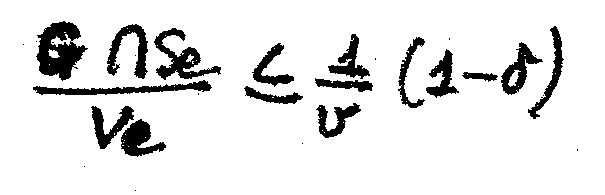
\includegraphics[width=\linewidth]{figures/gelfand-p000010-last-fraction-part01-original-r2.png}}
\expandafter\def\csname evidence-GELFAND-P000008-diagram-three-cells\endcsname{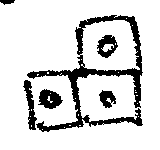
\includegraphics[width=\linewidth]{figures/gelfand-p000008-diagram-three-cells-part01-original-r1.png}}
\expandafter\def\csname evidence-GELFAND-P000009-diagram-corner-cluster\endcsname{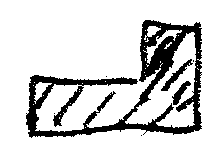
\includegraphics[width=\linewidth]{figures/gelfand-p000009-diagram-corner-cluster-part01-original-r1.png}}
\expandafter\def\csname evidence-GELFAND-P000009-diagram-coexistence-dome\endcsname{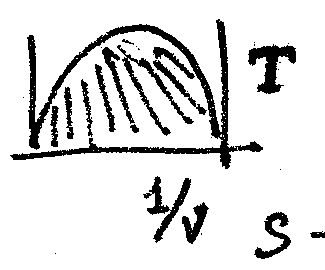
\includegraphics[width=\linewidth]{figures/gelfand-p000009-diagram-coexistence-dome-part01-original-r2.png}}
\newcommand{\GridWords}{Divided\\into subcubes}
\begin{document}
{\large\bfseries Gelfand seminar — chapter 1}\par
{\small Opening of the reader. Source frames 1–10. Text and formulas are typed; original details accompany every uncertain reading. Working excerpt; the complete chapter is still in preparation.}\par\medskip
\SourcePage{GELFAND-P000001}{unlabelled}
Monday, $21/\mathrm{IX}$.
Cartesian and Boolean products of groups.

``Hironaka: on resolution of singularities.''
\underline{Gelfand}

$A$ is a ring, $\mathcal{J}$ is a module over $A$.
\Unclear{GELFAND-P000001}{module-letter}{The letter for the module and ideal is rendered as $\mathcal{J}$; $\mathcal{I}$ or $J$ are possible.}

Blow-up --- ?
$M$ is a manifold; $D\subset M$.
[Beneath $D$:] a subset with singularities.

$M_0^H$ is the blow-up. Blowing-up.
The inverse image of $D$ is $D'$, a manifold of dimension $n-1$.
$D_0$ is $(n-1)$-dimensional.
\SourceFigure{GELFAND-P000001}{diagram-blowup}{Three enclosed drawings: at left a region with $D$; at upper right a region with $D'$ and the label $M_0^H$; at lower right a region and the label $M'_0$. The upper arrow points left; the lower oblique arrow also points left, with the label ``continuous map'' [source abbreviation: непр. отобр.]. The precise inner curves, labels and the connection of the lower region to the upper one require comparison with the scan.}
\Unclear{GELFAND-P000001}{blowup-notation}{The upper index on $M_0$ resembles $H$; the lower region's label resembles $M'_0$.}

The construction is Grothendieck's.
$A$ is a ring, $\mathcal{J}$ is a module.
\underline{Example.} $A$ is a ring of functions;
$\mathcal{J}$ is the ideal of functions taking the value $0$ on $D$.

One obtains a sheaf of rings and a sheaf of modules.
$A$ is a ring, $\mathcal{J}$ is an ideal.
Construct $X$, $O_X$ a sheaf of rings,
$\mathcal{J}_X$ a sheaf of ideals, so that
\begin{gather*}
 (A,\mathcal{J})\ \longleftarrow\ (X,O_X,\mathcal{J}_X).
\end{gather*}
[Beneath the arrow:] linear map.

$(A,\mathcal{J})$ is a sheaf generated by $1$ ideal.

$\mathcal{J}_X$ is invertible, i.e. an ideal of the ring:
$\exists f\in\mathcal{J}_X$ such that $O_Xf=\mathcal{J}_X$.
[Above the formula, an arrow to $\exists$:] generator.

(The ideal is principal if $\mathcal{J}$ is an ideal.)
Then the zero variety is $1$ equation.

$A$ is a ring, $\mathcal{J}$ is an ideal.
\underline{Typical example:} $R^2$, the ideal $=0$ at the origin.
\Unclear{GELFAND-P000001}{origin-example}{The next line: ``Gluing a projective line into $0$'' [source: Вклеив. в $0$ проект. прямой]; the beginning may read ``Оклеив.''.}

$A$, $\mathcal{J}$ are modules.
\begin{gather*}
 \mathcal{J}\otimes_A\mathcal{J},\qquad
 \mathcal{J}\otimes_A\mathcal{J}\otimes_A\mathcal{J},\ldots
\end{gather*}
[Above the groups of tensor products:] symmetric; symmetric.

Consider formal sums
\begin{gather*}
 \sum_{k=0}^{N}a_kz^k.
\end{gather*}
Add and multiply.
$x\otimes y=y\otimes x$.
\begin{gather*}
 a_0\in A,\qquad a_1\in\mathcal{J},\qquad
 a_2\in\mathcal{J}\otimes_A\mathcal{J}\quad\text{—}
\end{gather*}

\SourcePage{GELFAND-P000002}{unlabelled}
The ring of these sums is $S_A(\mathcal{J})$.
Consider homogeneous ideals
[inserted above the line:] (graded).
(Together with a polynomial it contains all its homogeneous components.)

Consider all homogeneous prime ideals in $S_A(\mathcal{J})$.
Выбр. [source abbreviation] ideals which contain all polynomials, starting with degree $1$.
\Unclear{GELFAND-P000002}{ideal-selection}{The end of the line after ``contain all'' is better read as ``polynomials, starting with degree $1$''; the middle strokes of the abbreviation ``нач.'' remain indistinct.}

The collection of ideals is $X$. (The Zariski topology.)
$O_X$, $\mathcal{J}_X$.
If $U$ is an open set, then $O_U$, $\mathcal{J}_U$.
\Unclear{GELFAND-P000002}{open-set-notation}{After ``then'', the first letter has the same form as $O_X$ above, the second as the ideal letter: $O_U$, $\mathcal{J}_U$; the latter may be $\mathcal{I}_U$.}

$S_A(\mathcal{J})$ is the whole ring.
The ring of fractions, numerators, denominators, not belonging to any of the ideals.
Localize the ring at this set.
Fractions of degree $1$: $\mathcal{J}_U$.
\Unclear{GELFAND-P000002}{fractions-sentence}{In the line about fractions, the abbreviations ``numerator--denominator'' and whether ``not belonging'' applies only to the denominator are unclear. No words are supplied from the meaning.}
[At right, two downward arrows:] Grothendieck --- blow up ideally.
\Unclear{GELFAND-P000002}{margin-grothendieck}{The right-hand note reads ``Grothendieck --- blow up ideally''; the last word may be ``идеально'' [ideally] or ``идеалы'' [ideals].}

$A$ is the ring of polynomials in $2$ variables.
$\mathcal{J}$ is the ideal of polynomials with $P(0,0)=0$.
\begin{gather*}
 A=\{P(x,y)\},\qquad
 \mathcal{J}=P(x,y)=a_1x+b_1y+\cdots .
\end{gather*}
\begin{gather*}
 \mathcal{J}\otimes_A\mathcal{J}\ \longleftrightarrow
 \{a_2x^2+2b_2xy+cy^2+\cdots\}.
\end{gather*}
\Unclear{GELFAND-P000002}{quadratic-coefficients}{The coefficients in the quadratic polynomial read $a_2$, $2b_2$, $c$; the index on $c$ and the shape of the thick two-headed arrow are uncertain.}

Because of the interchange, one obtains the same as the square of the ideal.
Then --- the ideal of polynomials equal to $0$ at this point.
What will it blow up into? ?

\begin{gather*}
 \sum P_k(x,y)z^k,\qquad P_k(x,y)=ax^k+\cdots .
\end{gather*}
[At right:] Graded $\Sigma$ of tensor products.
\begin{gather*}
 A=\{P_0(x,y)\}\longrightarrow S_A(\mathcal{J}),\qquad
 P_0(x,y)\sim P_0(x,y).
\end{gather*}
The set of prime ideals obtained from the ideal $P(0,0)=0$.
\begin{gather*}
 S_A\sim\sum P_kz^k,\qquad P_k\in\mathcal{J}^k,\qquad
 K\sim\sum P_kz^k.
\end{gather*}
It suffices to find the max. ideals of the quotient ring ---
(to find the ideals containing the given one).
\begin{gather*}
 S_A/K\ \longleftrightarrow\ a_0+(a_1x-b_1y)z+\cdots .
\end{gather*}
\Unclear{GELFAND-P000002}{last-sign}{In the last formula a minus is visible before $b_1y$, although the next scan has a plus. The visible minus is retained; the direction of the thick arrow is also uncertain.}

\SourcePage{GELFAND-P000003}{2}
All homogeneous max. ideals in it will be the points of the extension.
There is no constant term (then also $1$).
\begin{gather*}
 (a_1x+b_1y)z.
\end{gather*}
Only $1$ linear combination of $x$ and $y$.
(Not $2$, since then all.)

The ideals determine directions in the plane
(замк. [source abbreviation] with all possible directions --- the $\sigma$-process).
\Unclear{GELFAND-P000003}{directions}{The abbreviations in parentheses read ``замк. всеми возм. напр.''; neither the first word nor the meaning of the sign $\sigma$ is asserted.}
\Needspace{48mm}\underline{Problem.} In the space
[cancelled:] \Unclear{GELFAND-P000003}{cross-cancellation}{The cancelled word before the drawing is illegible.}
\par\smallskip\noindent\begin{minipage}{\linewidth}\begin{minipage}[t]{.47\linewidth}\centering\vspace{0pt}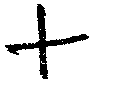
\includegraphics[width=30mm]{figures/gelfand-p000003-cross-diagram-original-r1.png}\par{\scriptsize Original diagram}\end{minipage}\hfill\begin{minipage}[t]{.49\linewidth}\centering\vspace{0pt}\begin{tikzpicture}[scale=0.5]
 \draw (-0.8,0)--(0.8,0);
 \draw (0,-0.7)--(0,0.8);
\end{tikzpicture}\par{\scriptsize Typeset recreation}\end{minipage}\end{minipage}\par\smallskip
What results from gluing it in?
\begin{gather*}
 z=0,\qquad xy=0,\qquad \mathcal{J}=(z,xy).
\end{gather*}
[A line is drawn beneath the system.]

\underline{Dobrushin.}
[Cancelled before ``Find'':] \Unclear{GELFAND-P000003}{ising-cancellation}{The cancelled beginning of the line cannot be read confidently.}
Find an example of a gas in which phase transitions occur.
A cube of the integer lattice.
$\ell$ is the length. $V_\ell=\ell^\nu$.
$N$ points, $N<V_\ell$.
They can occupy positions on the lattice
$\theta=(x_1,\ldots,x_N)$.
\Unclear{GELFAND-P000003}{configuration-letter}{The configuration sign is rendered as $\theta$; the handwritten sign also resembles $b$ or Cyrillic ``в''.}

The Ising model.
[Before the formula, a densely cancelled sign:]
\Unclear{GELFAND-P000003}{energy-cancellation}{The separate cancelled sign before $U(\theta)$ is illegible.}
\begin{gather*}
 U(\theta)=-\frac12\sum_{i\ne j}u(x_i,x_j),\qquad
 u=\begin{cases}
 0&\text{in the other cases},\\
 1;&\rho(x_i,x_j)=1.
 \end{cases}
\end{gather*}
$u(\theta)$ is the number of pairs of neighboring points.
\Unclear{GELFAND-P000003}{energy-case}{In the condition for the second branch a sign resembling $\rho$ is visible; the semicolon after $1$ is retained. In the caption below, the first letter resembles lowercase $u$ rather than $U$.}

The basic axiom is the Gibbs distribution.
\begin{gather*}
 \mathsf{P}(B)=
 \frac{\displaystyle\sum_{\theta\in B}\exp\{-U(\theta)/T\}}
 {Z(V_\ell,N)},\qquad T>0\text{ --- temperature.}
\end{gather*}
[Beneath the denominator:] normalizing factor.
\begin{gather*}
 Z(\ell,N)=\sum_{\theta\in\mathcal{B}}\exp\{-U(\theta)/T\}.
\end{gather*}
\Unclear{GELFAND-P000003}{partition-domain}{The denominator in the first formula reads $Z(V_\ell,N)$, the next line $Z(\ell,N)$; the set sign beneath the sum resembles $\mathcal{B}$. The notation is not adjusted for consistency.}

The molecules attract one another.
([Two filled signs with arrows:] neighbors $>$ their probability.)
\Unclear{GELFAND-P000003}{attraction-note}{In parentheses after ``The molecules attract'', there are filled signs and arrows; the reading ``neighbors $>$ their probability'' is uncertain.}
$B\subset\mathcal{B}$ is a collection of configurations.
\begin{gather*}
 p(\theta)=\frac{\exp\{-U(\theta)/T\}}{Z(\ell,N)}.
\end{gather*}
Take the limit $\ell\to\infty$; the cube expands to $\infty$.
$N_\ell$ depends on $\ell$.
[A cancelled sign before the fraction:]
\Unclear{GELFAND-P000003}{density-cancellation}{The cancelled sign before $V_\ell/N_\ell$ is illegible.}
\begin{gather*}
 \frac{V_\ell}{N_\ell}=v=\mathrm{const}.
\end{gather*}
The lattice grows.
One can show that
\begin{gather*}
 \frac1{N_\ell}\log Z(\ell,N_\ell)\longrightarrow f(v,T).
\end{gather*}

\SourcePage{GELFAND-P000004}{unlabelled}
\begin{gather*}
 p(v,T)=T\frac{\partial f}{\partial v}\qquad\text{by definition.}
\end{gather*}
\Unclear{GELFAND-P000004}{pressure-letter}{The heavily written first argument of $p$ resembles $v$; no minus is visible before the derivative, and none is supplied.}

Phase transition.
As for $f$: it is a monotone, convex function of $v$.
Therefore $p>0$, and $p$ is a monotone function of $v$.
Phase transition: $p(v,T)$ has a flat segment.
\SourceFigure{GELFAND-P000004}{diagram-phase-point}{In the upper right-hand field is a bent, S-like curve with an almost horizontal middle segment and an arrow toward it; the caption reads ``points of phase transition'' [source abbreviation: точки фаз. перехода]. Precise axes and points in the original drawing are not identified confidently.\par\smallskip\centering\resizebox{.93\linewidth}{!}{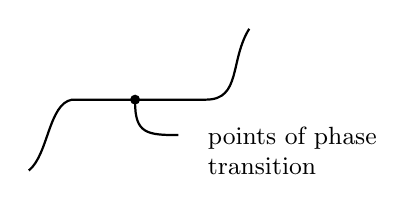
\begin{tikzpicture}[x=1cm,y=1cm]
\draw[thick] (0,0)..controls(.25,.2)and(.25,.85)..(.55,.9)--(2.25,.9)..controls(2.7,.9)and(2.55,1.4)..(2.8,1.8);
\fill(1.35,.9)circle(1.8pt);
\draw[thick](1.35,.87)..controls(1.35,.47)and(1.5,.45)..(1.9,.45);
\node[anchor=west,align=left,font=\small]at(2.15,.25){\PhaseWords};
\end{tikzpicture}}\par{\scriptsize Typeset sketch; limitations are recorded in the note.}\par}
There is a physical hypothesis: $1$ transition segment.

\SourceFigure{GELFAND-P000004}{diagram-cancelled-graph}{At left is a graph with vertical and horizontal axes, $0$ and $\infty$ by the horizontal axis. Several curves and straight lines are heavily crossed out; the precise cancelled curve and the vertical label need comparison.\par\smallskip\centering\resizebox{.93\linewidth}{!}{\begin{tikzpicture}[x=1cm,y=1cm]
\draw[thick](0,1.75)--(0,0)--(3.6,0);
\node[below]at(0,-.05){$0$};\node[below]at(3.6,-.05){$\infty$};
\end{tikzpicture}}\par{\scriptsize Partial recreation: secure axes only; cancelled curves remain unresolved.}\par}
\SourceFigure{GELFAND-P000004}{diagram-pressure-plateau}{Neighboring drawing at right: a clean descending curve with a flat segment. This is a separate graph, not a reconstruction of the cancelled drawing at left.\par\smallskip\centering\resizebox{.9\linewidth}{!}{\begin{tikzpicture}[scale=0.7]
 \draw (0,0)--(4.6,0);
 \draw (0,0)--(0,2.3);
 \draw (0.2,2.5).. controls (0.9,2.4) and (0.5,1.25)..(1.2,1.15)
 --(2.4,1.15).. controls (2.9,1.05) and (2.7,0.45)..(4,0.35);
 \node at (-0.1,-0.4) {$0$};
 \node at (4.6,-0.4) {$\infty$};
\end{tikzpicture}}\par{\scriptsize Existing typeset recreation.}}
A flat segment occurs for sufficiently small $T$ ($<T_{\text{crit}}$).

It admits an explicit solution for $n=1$.
$Z$ and $f(v,T)$ are calculated.
There are no phase transitions, which is considered physically natural.

\underline{$n=2$.} \underline{Onsager.}
$f(v,T)$ is calculated for particular $v$ and $T$.
A discontinuity of the derivative corresponds to phase transitions.
\SourceFigure{GELFAND-P000004}{diagram-onsager}{A graph with the $T$ axis upward, the $v$ axis to the right, and the label $1/2$ beneath a vertical through the vertex. The curve rises from the left to the vertex and descends to the right; the vertical line passes through the vertex, with a short wavy segment to its right. The precise geometry and the meaning of the wavy branch have not been established.\par\smallskip\centering\resizebox{.93\linewidth}{!}{\begin{tikzpicture}[x=1cm,y=1cm]
\draw(0,0)--(4.6,0);\draw(0,0)--(0,2.3);
\node[left]at(0,2.3){$T$};\node[below]at(4.6,0){$v$};
\draw(2.2,-.05)--(2.2,2.65);\node[below]at(2.2,-.12){$1/2$};
\draw[thick](.7,-.02)..controls(1.25,.35)and(1.85,.95)..(2.2,1.35)..controls(2.4,1.1)and(3.05,.55)..(3.45,.18);
\draw(1.05,.18)..controls(1.5,.54)and(1.9,1)..(2.17,1.35);
\fill(2.2,1.35)circle(1.5pt);
\draw[thick](2.32,1.4)..controls(2.5,1.62)and(2.63,1.33)..(2.78,1.42)..controls(2.86,1.47)and(2.98,1.56)..(3.03,1.61);
\end{tikzpicture}}\par{\scriptsize Typeset sketch; limitations are recorded in the note.}\par}

Kac, Helfand.
Exact, in explicit form, for some cases [source endings: точн. в яв. виду для нек-рых случаях].
\Unclear{GELFAND-P000004}{kac-helfand-note}{After another enlargement, the line reads ``точн. в яв. виду для нек-рых случаях''; the endings may instead be ``виде'' and ``случаев''. The ungrammatical reading is not corrected automatically.}

\SourceFigure{GELFAND-P000004}{diagram-subcube}{A large square with a smaller outlined region inside; $H$ at its center and $h$ above the smaller region. The small contour is partly square and partly rounded; its precise boundary has not been reconstructed.\par\smallskip\centering\resizebox{.93\linewidth}{!}{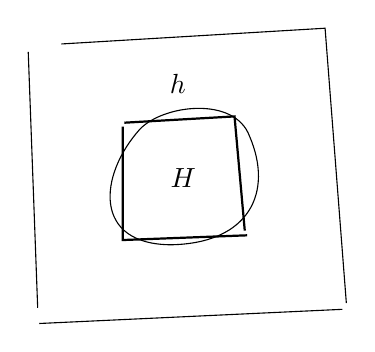
\begin{tikzpicture}[x=1cm,y=1cm]
\draw(.3,3.45)--(3.65,3.65)--(3.92,.16);\draw(3.87,.08)--(.02,-.1);\draw(0,.1)--(-.12,3.35);
\draw[thick](1.1,2.45)--(2.5,2.53)--(2.63,1.08);\draw[thick](2.66,1.02)--(1.08,.96)--(1.08,2.4);
\draw(1.3,2.37)..controls(1.6,2.68)and(2.5,2.79)..(2.69,2.28)..controls(3,1.56)and(2.68,.92)..(1.7,.9)..controls(.7,.9)and(.77,1.78)..(1.3,2.37);
\node at(1.85,1.75){$H$};\node at(1.78,2.94){$h$};
\end{tikzpicture}}\par{\scriptsize Typeset sketch; limitations are recorded in the note.}\par}
\begin{gather*}
 \frac{\mu_H}{h^\nu}.
\end{gather*}
$\mu_H$ is the number of particles in $H$ --- a subcube.
$\nu$ is the dimension.
\begin{gather*}
 \frac{\mu_H}{h^\nu}=\frac1v\qquad\text{as in the whole space.}
\end{gather*}
\underline{Law of large numbers.}
\begin{gather*}
 \mathsf{P}\left\{\frac{\mu_H}{h^\nu}-\frac1v\,\middle|\,>\varepsilon\right\}
 \longrightarrow0.
\end{gather*}
\Unclear{GELFAND-P000004}{probability-bar}{In the probability formula the right vertical bar before $>\varepsilon$ is visible; a left bar before the fraction has not been read confidently. No matching bar is silently supplied.}
\begin{gather*}
 \ell\to\infty,\qquad H\to\infty,\qquad
 d<\frac h\ell<1-d,\qquad d>0.
\end{gather*}
\Unclear{GELFAND-P000004}{bottom-mark}{At the lower right edge a small sign resembles ``2'' or a broken-off letter; it has not been adopted as a page number.}
\Incomplete{GELFAND-P000004}{margin-left}{Along the extreme left edge is a narrow strip of neighboring handwritten text, cropped to isolated endings and strokes; no connected text can be read.}


\SourcePage{GELFAND-P000005}{3}
If this does \underline{not} hold, a phase transition takes place.
\Unclear{GELFAND-P000005}{physical-meaning-heading}{Нагл. [candidate abbreviation; the middle strokes are not fully distinguishable]} meaning. $2$ phases coexist; the particles are distributed unevenly ---
--- liquid and gas.
[Above the line:] (law of large numbers).
[Inserted above ``phase transition'', with a bracket:] absence.
(A closely related condition is necessary and sufficient for a phase transition
\begin{gather*}
 \mathsf{P}_\ell\left\{\left|\frac{\mu_H}{h^\nu}-\frac1v\right|>\varepsilon\right\}
 =O(e^{-N\beta}).
\end{gather*}
\Unclear{GELFAND-P000005}{exponential-rate}{The exponent of $e$ contains a heavily written sign before $\beta$; the candidate is $-N\beta$, but $N$ is obscured by overlapping strokes. The parenthesis opened before ``A closely related'' is not clearly closed in the scan.}
[At right:] $N$ is the number of particles.

Calculate the probability that
\begin{gather*}
 \mathsf{P}\{\mu_H=k\}=Z^{-1}
 \sum_{\theta\in\mathcal{B}_k}\exp\{-U(\theta)/T\}.
\end{gather*}
Over configurations in which $H$ contains $k$ particles.
$\theta$ is a configuration of $N$ particles.
$\theta\in\mathcal{B}_k$.
Then $\theta=(\theta_1,\theta_2)$.
$\theta_1$ is a configuration of $k$ particles in $H$.
$\theta_2$ is a configuration of $(N-k)$ particles in $\overline H$.
\Unclear{GELFAND-P000005}{complement-label}{The upper bar on $H$ in the line about $\theta_2$ is not completely distinct; the candidate is $\overline H$.}
\begin{gather*}
 U(\theta)=U(\theta_1)+U(\theta_2)+\gamma(\theta).
\end{gather*}
$U(\theta_1)$ is the interaction inside.
$U(\theta_2)$: neighbors outside.
$\gamma(\theta)$ is the interaction across the surface.
$\gamma(\theta)$ can be neglected asymptotically.
(Across the boundary: of the order of the number of boundary points)
$V^{\nu-1/\nu}$ as $N\to\infty$.
$k\sim dN$.
\Unclear{GELFAND-P000005}{boundary-exponent}{The exponent on $V$ looks like $\nu-1/\nu$, without a confidently distinguishable common numerator. It has not been changed automatically to $(\nu-1)/\nu$.}
\begin{gather*}
 |\gamma(\theta)|\le CN^{\frac{\nu-1}{\nu}}.
\end{gather*}
\begin{align*}
 \sum\exp\{-U(\theta)/T\}
 &=\sum_{\theta\in\mathcal{B}_k}\exp\{-U(\theta_1)/T\}
 \exp\{-U(\theta_2)/T\}\\
 &\qquad\times
 \exp\{\theta N^{2/3}\}
 =
\end{align*}
\Unclear{GELFAND-P000005}{theta-factor}{The letter before $N^{2/3}$ resembles $\theta$ or $\Theta$; below, the same letter is glossed as ``bounded parameter''. It may differ from the configuration sign.}
$\theta$ is a bounded parameter.
\begin{gather*}
 =\exp\{\theta N^{2/3}\}
 \sum_{\theta_1}\exp\{-U(\theta_1)/T\}
 \sum_{\theta_2}\exp\{-U(\theta_2)/T\}.
\end{gather*}
[Beneath the first sum:] configurations.


\SourcePage{GELFAND-P000006}{unlabelled}
Factor $1$: $Z$, calculated for the subcube.
Factor $2$ — ditto — $Z$ for the outer cube.
\begin{gather*}
 \mathsf{P}\{\mu_H=k\}
 =\frac{Z(H,k)Z(\overline H,N-k)}{Z(V,N)}
 \exp\{\theta N^{2/3}\}.
\end{gather*}
[Asterisk.]
Apply to them the asymptotic formula
\begin{gather*}
 Z(V,N)\approx\exp\{-Nf(v,T)\},
\end{gather*}
\begin{gather*}
 Z(H,k)=\exp\{-kf(h^3/k,T)\}.
\end{gather*}
\Unclear{GELFAND-P000006}{subcube-power}{The numerator of the argument of $f$ in this line visibly has exponent $3$ on $h$, although $\nu$ is used later. The written $h^3$ is retained.}
It can also be proved for well-behaved regions (not a cube).
The limiting formula does not depend on the region's shape.
\begin{gather*}
 Z(\overline H,N-k)=
 \exp\{-(N-k)f((\ell^3-h^3)/(N-k),T)\}.
\end{gather*}
Substitute there under the assumption that $f$ has a linear segment.
If $f$ has a linear segment (the derivative has a horizontal one),
then terms cancel and we obtain
\begin{gather*}
 \frac1N\log\mathsf{P}\{\mu_H=k\rho\}\longrightarrow
 \begin{cases}
 0&\text{only at }\rho=1/v\text{ (if there is no linear segment)},\\
 0&\rho\in\text{ the linear segment}.
 \end{cases}
\end{gather*}
[Cancelled by the second branch:]
\Unclear{GELFAND-P000006}{limit-notation}{The event's argument looks like $\mu_H=k\rho$, but the final sign may be $\theta$ or $\delta$. The density letter at right resembles $\rho$. The cancelled text above the second branch has not been read.}
\SourceFigure{GELFAND-P000006}{diagram-limit-step}{At right of the second branch of the limit is a small stroke: from the lower left, a line rises almost vertically, then runs almost horizontally to the right, and rises again at the right end. Separate axes, arrows and labels have not been established; the sketch's mathematical meaning requires the original image.\par\smallskip\centering\resizebox{.93\linewidth}{!}{\begin{tikzpicture}[x=1cm,y=1cm]
\draw[thick] (0,0)..controls(.2,.65)and(.35,1.2)..(.65,1.35)--(2.4,1.4)--(2.45,2.15);
\end{tikzpicture}}\par{\scriptsize Visible stroke; no axes or values supplied.}\par}
$\mathsf{P}\to0$ exponentially.
($1/v$ follows from the \underline{convexity} of $f$.)

Arrangement of particles.
Its boundary; around each particle a cube of side $1$.
$\Gamma'(\theta)$ is the boundary of the occupied region.
$\Gamma(\theta)$ is the length
[inserted below:] area.
\SourceFigure{GELFAND-P000006}{diagram-cell-clusters}{Inside a square frame, a vertical shaded chain is at left; its internal divisions merge with the hatching. At right, three cells form a corner: two below and one above the left cell. The left cell count is unresolved.\par\smallskip\centering\resizebox{.93\linewidth}{!}{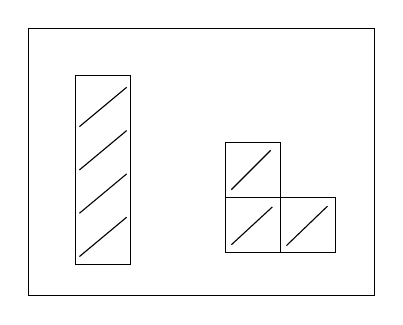
\begin{tikzpicture}[x=1cm,y=1cm]
\draw(0,0)rectangle(4.4,3.4);
\draw(.6,.4)rectangle(1.3,2.8);
\draw(2.5,.55)rectangle(3.2,1.25);\draw(3.2,.55)rectangle(3.9,1.25);\draw(2.5,1.25)rectangle(3.2,1.95);
\foreach \y in{.5,1.05,1.6,2.15}{\draw(.65,\y)--(1.25,\y+.5);}
\draw(2.58,.65)--(3.1,1.13);\draw(3.28,.64)--(3.8,1.14);\draw(2.58,1.35)--(3.08,1.85);
\end{tikzpicture}}\par{\scriptsize Partial left-chain outline; internal divisions unresolved. Three-cell corner at right.}\par}
\underline{Replace} the Gibbs probability.
\begin{gather*}
 \mathsf{P}(\theta)=
 \frac{\exp\{-U(\theta)/T\}}{\sum\exp\{-U(\theta)/T\}}
 =\frac{\exp\{-\Gamma'(\theta)/(2T)\}}
 {\sum\exp\{-\Gamma'(\theta)/(2T)\}}.
\end{gather*}
\Unclear{GELFAND-P000006}{gamma-prime}{The prime on $\Gamma$ in the two exponents after the equality is not completely clear; the visible letter resembles $\Gamma'$ or $\Gamma$.}
[At right:] $2\nu-\delta$.
Unoccupied \underline{squares} $\Gamma'(\theta)$.
[Inserted:] at neighbors.
\begin{gather*}
 -U(\theta)\ \ge\ \sum(2\nu-\delta)
 =2\nu N-\sum_{\Gamma'(\theta)}\delta.
\end{gather*}
\Unclear{GELFAND-P000006}{energy-bound}{The sign after $-U(\theta)$ is written over another sign: candidates are $\ge$, $\le$, and $=$. The sign before the final sum and the sum's index may belong to another term; the visible candidate is retained without a mathematical correction.}


\SourcePage{GELFAND-P000007}{4}
($U(\theta)$ is minus the number of neighbors.)
A smaller boundary makes an arrangement more favorable.
Force them into one corner, but this is unfavorable
(there are few such arrangements in all).
A finite number of clumps.
(Inside the gas: liquid.)
\SourceFigure{GELFAND-P000007}{diagram-small-clusters}{Small square drawing at right: two filled regions and small strokes in the upper left corner. The number and meaning of the small strokes are unclear.\par\smallskip\centering\resizebox{.93\linewidth}{!}{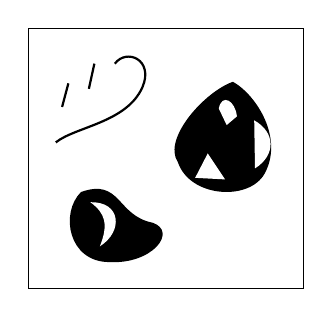
\begin{tikzpicture}[x=1cm,y=1cm]
\draw(0,0)rectangle(3.5,3.3);
\draw[thick](.35,1.85)..controls(.6,2.05)and(1.25,2.1)..(1.45,2.55)..controls(1.6,2.9)and(1.25,3.05)..(1.1,2.85);
\draw[thick](.43,2.3)--(.51,2.6);\draw[thick](.77,2.53)--(.84,2.85);
\fill(2.6,2.62)..controls(2.9,2.45)and(3.25,1.9)..(3,1.45)..controls(2.8,1.1)and(2.05,1.15)..(1.9,1.6)..controls(1.7,1.9)and(2.25,2.5)..(2.6,2.62);
\fill[white](2.42,2.28)..controls(2.46,2.48)and(2.63,2.38)..(2.65,2.18)--(2.52,2.07)--cycle;
\fill[white](2.87,2.13)..controls(3.14,1.98)and(3.15,1.69)..(2.88,1.52)--cycle;
\fill[white](2.28,1.71)--(2.5,1.38)--(2.12,1.4)--cycle;
\fill(.67,1.22)..controls(1.18,1.4)and(1.12,.92)..(1.58,.83)..controls(1.9,.72)and(1.58,.3)..(1.03,.33)..controls(.51,.33)and(.4,.95)..(.67,1.22);
\fill[white](.79,1.09)..controls(1.18,1.1)and(1.21,.72)..(.91,.53)..controls(1.02,.81)and(.98,.95)..(.79,1.09);
\end{tikzpicture}}\par{\scriptsize Partial sketch of patches and visible marks; small strokes remain uninterpreted.}\par}
And this contradicts the law of large numbers.

\SourceFigure{GELFAND-P000007}{diagram-cycles}{A large rectangular frame at left contains three separate rounded regions with inner contours and shaded parts; one has a central island. The precise cycles, shading and nesting require the original image.\par\smallskip\centering\resizebox{.93\linewidth}{!}{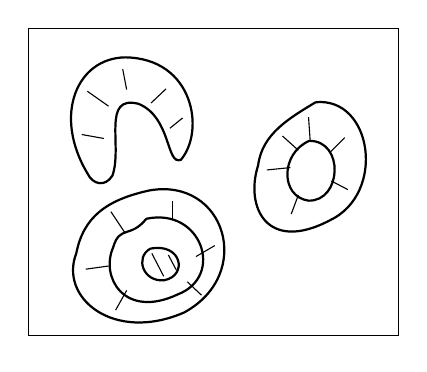
\begin{tikzpicture}[x=1cm,y=1cm]
\draw(0,0)rectangle(4.7,3.9);
\draw[thick](.75,2.06)..controls(.31,2.8)and(.62,3.52)..(1.23,3.53)..controls(2.1,3.52)and(2.25,2.6)..(1.94,2.23)..controls(1.75,2.15)and(1.82,2.77)..(1.4,2.94)..controls(.93,3.06)and(1.2,2.4)..(1.07,2.03)..controls(.98,1.88)and(.82,1.91)..(.75,2.06);
\draw(.68,2.55)--(.96,2.5);\draw(.75,3.1)--(1.02,2.91);\draw(1.2,3.38)--(1.25,3.12);\draw(1.75,3.13)--(1.56,2.95);\draw(1.96,2.76)--(1.8,2.63);
\draw[thick](3.65,2.96)..controls(4.37,3.03)and(4.55,1.8)..(3.83,1.46)..controls(3.03,1.04)and(2.75,1.63)..(2.92,2.16)..controls(2.97,2.56)and(3.32,2.76)..(3.65,2.96);
\draw[thick](3.57,2.47)..controls(4.02,2.47)and(3.98,1.7)..(3.56,1.71)..controls(3.2,1.76)and(3.2,2.31)..(3.57,2.47);
\draw(3.03,2.1)--(3.33,2.13);\draw(3.23,2.53)--(3.43,2.35);\draw(3.56,2.77)--(3.58,2.48);\draw(4.02,2.51)--(3.84,2.33);\draw(4.06,1.85)--(3.85,1.96);\draw(3.34,1.54)--(3.43,1.78);
\draw[thick](1.54,1.84)..controls(2.5,2.01)and(2.88,.78)..(1.98,.29)..controls(1.08,-.1)and(.39,.48)..(.61,1.04)..controls(.7,1.5)and(.99,1.72)..(1.54,1.84);
\draw[thick](1.5,1.48)..controls(2.2,1.63)and(2.5,.75)..(1.9,.52)..controls(1.22,.2)and(.91,.74)..(1.08,1.12)..controls(1.16,1.4)and(1.3,1.23)..(1.5,1.48);
\draw[thick](1.55,1.1)..controls(1.95,1.18)and(2.03,.76)..(1.73,.7)..controls(1.46,.67)and(1.35,.99)..(1.55,1.1);
\draw(1.57,1.04)--(1.72,.75);\draw(1.78,1.02)--(1.88,.83);
\draw(.73,.84)--(1.02,.88);\draw(1.05,1.57)--(1.23,1.3);\draw(1.83,1.7)--(1.83,1.48);\draw(2.37,1.14)--(2.13,1);\draw(2.2,.51)--(2.02,.68);\draw(1.11,.32)--(1.25,.57);
\end{tikzpicture}}\par{\scriptsize Nesting sketch, retaining the lower opening of the upper-left group.}\par}
The whole boundary splits into connected cycles.
Each arrangement has its own number.
Number them
\begin{gather*}
 \Gamma_1(\theta)\ge\Gamma_2(\theta)\ge\cdots,\qquad
 \Gamma(\theta)=\sum_i\Gamma_i(\theta).
\end{gather*}
An arrangement is special if $\exists N<\infty$, $D<\infty$, $\delta>0$.
\Unclear{GELFAND-P000007}{special-arrangement-count}{In this line the first finite parameter resembles $N$, whereas the later summation limit resembles $M$. This difference is not smoothed out.}
\begin{gather*}
 1)\quad\sum_{i=1}^{M}\Gamma_i(\theta)
 \le D\ell^{\frac{\nu-1}{\nu}}.
\end{gather*}
[Beneath the sum:] Large.
Of the order of the boundary length. (Almost the whole cube.)
\Unclear{GELFAND-P000007}{large-cycles-power}{The exponent on $\ell$ in the first condition is written as a fraction, read as $(\nu-1)/\nu$; in GELFAND-P000010 the analogous line has $\nu-1$. The difference is retained.}
\begin{gather*}
 2)\quad\text{all the others small}\qquad
 \sum_{i=1}^{M}\bigl(\Gamma_i(\theta)\bigr)^{\frac\nu{\nu-1}}.
\end{gather*}
\Unclear{GELFAND-P000007}{small-cycles-sum}{The visible limits of the second sum look like $1$ and $M$, although the caption says ``all the others small''. No condition is visible after the sum; none is supplied from the later scan.}
[Dividing line.]

$24/\mathrm{IX}$.
Thursday. $16$ h, room $13$-$11$.
Prof. Segal (USA).
\underline{Theory of functions in infinite-dimensional space.}
\begin{gather*}
 +\Box\varphi=m^2\varphi+g\varphi^3.
\end{gather*}
\begin{gather*}
 F_f(\varphi)=\int(-\Box+m^2)f\varphi
 +g\int\varphi^3 f.
\end{gather*}
[Above $\varphi^3$:] $\varphi$ — мн. [source abbreviation].
$\varphi$ [arrow] $C_0^\infty$ — functions.
\Unclear{GELFAND-P000007}{field-margin}{Above the note at right are the visible words ``б, ф-й на'' [fragment: functions on] and an arrow toward $C_0^\infty$; this may define the function $\varphi$ on the space of test functions, but no text is supplied.}
$g$ is fixed.
$F_f\in\Phi$ is a nonlinear functional of $\varphi$.
$\Phi$ is a ring; one can multiply $F_1(\varphi)F_2(\varphi)$.
Take the ideal generated by $(F_f:f\in C_0^\infty)$ — $\Omega$.
\Unclear{GELFAND-P000007}{ideal-signature}{The index on $F$ in the ideal's definition resembles $f$; the source sign after the parenthesis is $\Omega$ or a calligraphic $J$.}
Let $p=\Phi/\Omega$ be the function ring on the manifold of solutions
of the given partial differential equation.
To obtain a solution $(1)$ $\overset{\mathrm{def}}=$
a point of the space of maximal ideals of the ring $p$.
An ordinary solution $\varphi_0$ [a check mark above the word] is assigned a maximal ideal: consider the map
\begin{gather*}
 F\longrightarrow F(\varphi_0),
\end{gather*}
a homomorphism into $\Phi$,
$F_f$ is zero on the ideal $\Omega$.
This is a homomorphism of the quotient ring as well, i.e. a maximal ideal.
\Unclear{GELFAND-P000007}{evaluation-target}{After ``a homomorphism into'', the visible letter resembles $\Phi$, although its meaning might suggest a field. The letter candidate is retained rather than corrected mathematically.}


\SourcePage{GELFAND-P000008}{unlabelled}
A maximal ideal is a generalized solution of a nonlinear equation.
The algebraic case.
\begin{gather*}
 f_1(x_1,\ldots,x_n)=0,\qquad
 f_k(x_1,\ldots,x_n)=0.
\end{gather*}
Solutions in terms of a ring: in the ring of all polynomials.
The ideal generated by these functions is $p$, and the quotient ring is
$\Phi/p$.
\Unclear{GELFAND-P000008}{algebra-ring-letter}{In the fraction, the numerator resembles $\Phi$, $P$, or a heavily written $A$; the candidate $\Phi$ is retained.}
$\Phi$ — all equations.
This is the ring of algebraic functions.
A point, the value at the point, is precisely a maximal ideal.
In the algebraic case, conversely as well.
Analogy: linear oscillations.
\begin{gather*}
 \int f(-\Box\varphi\ldots)\,dx.
\end{gather*}
\Unclear{GELFAND-P000008}{linear-oscillation}{The part of the integral after $-\Box$ looks like $\varphi\ldots$, but the letter is partly inked over.}
And the corresponding ideal.

\underline{Dobrushin.}
$\nu=2,3$.
$V_\ell=\ell^\nu$, $N<V_\ell$,
$\theta=(x_1,\ldots,x_N)$.
\SourceFigure{GELFAND-P000008}{diagram-three-cells}{Original and existing typeset recreation.\par\smallskip\centering\resizebox{.93\linewidth}{!}{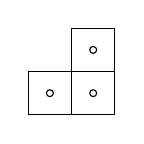
\begin{tikzpicture}[scale=0.55]
 \draw (0,0) rectangle (1,1);
 \draw (1,0) rectangle (2,1);
 \draw (1,1) rectangle (2,2);
 \draw (0.5,0.5) circle (0.08);
 \draw (1.5,0.5) circle (0.08);
 \draw (1.5,1.5) circle (0.08);
\end{tikzpicture}}}
$\Gamma(\theta)$ is the boundary length.
$U(\theta)$ is the number of neighbors (pairs of neighbors).
The Gibbs distribution
\begin{gather*}
 p(\theta)=
 \frac{\exp\{U(\theta)/T\}}
 {\displaystyle\sum_{\theta\in\mathcal{B}(V_\ell,N)}\exp\{U(\theta)/T\}}
 =\frac{\exp\{-\Gamma(\theta)/(2T)\}}
 {\displaystyle\sum_\theta\exp\{-\Gamma(\theta)/(2T)\}}.
\end{gather*}
[Beneath the first sum:] all arrangements.
\begin{gather*}
 (\text{since }2U(\theta)=2\nu N-\Gamma(\theta)).
\end{gather*}
\underline{Phase transition.}
Let the lattice grow, $\ell\to\infty$,
and let $N_\ell\to\infty$.
The limit $V_\ell/N_\ell\to v$ is the specific volume.
It turns out that
\begin{gather*}
 \frac1N\log\sum_\theta\exp\{U(\theta)/T\}\longrightarrow f(v,T).
\end{gather*}
\Unclear{GELFAND-P000008}{name-van-hove}{Beneath the limit the name reads ``Ван Хов'' or ``Ванхов'' [Van Hove]; the middle and ending are heavily overwritten.}
$(v,T)$ is called a point of phase transition if
\begin{gather*}
 \frac{\partial f(v,T)}{\partial v}=0
 \quad\text{in some neighborhood at }T=\mathrm{const}.
\end{gather*}
\Unclear{GELFAND-P000008}{temperature-relation}{Between $T$ and const, the sign resembles $=$ or $\ne$; the candidate $=$ is retained, but the reading is not asserted.}
\Incomplete{GELFAND-P000008}{margin-left}{At the extreme left edge is a narrow cropped column of handwritten endings from neighboring text; continuous words cannot be recovered.}


\SourcePage{GELFAND-P000009}{5}
(Since the function is linear; a priori it is convex.)
\begin{gather*}
 Q(T)=\frac{S_\nu e(1-e^{-1/(2T)})}
 {3(1+e^{-\nu/T})}
 \sum_{k=2\nu}^{\infty}3\exp\{-1/(2T)\}^{k}
 k^{\frac\nu{\nu-1}}.
\end{gather*}
[After the first equality, a cancelled fragment:]
\Unclear{GELFAND-P000009}{q-formula}{The cancelled sign after $=$ is illegible. In the numerator, the factor after $S_\nu$ resembles $e$; the upper summation limit resembles $\infty$ or a double stroke. The exponent $k$ may apply to the factor $3$ as well, but in the scan it stands by the closing brace. The variants are not replaced with a standard formula.}
$S_\nu$ is the volume of a $\nu$-dimensional sphere with surface $1$.
\begin{gather*}
 S_2=\frac1{4\pi},\qquad S_3=\frac1{C\sqrt\pi}.
\end{gather*}
\Unclear{GELFAND-P000009}{sphere-constant}{The first factor in the denominator of $S_3$ resembles $C$, $c$, or $6$; the written $C$ is only a candidate.}
If
\begin{gather*}
 Q(T)<\frac1v<1-Q(T),
\end{gather*}
then a phase transition takes place.
\SourceFigure{GELFAND-P000009}{diagram-coexistence-dome}{Original and existing typeset recreation.\par\smallskip\centering\resizebox{.93\linewidth}{!}{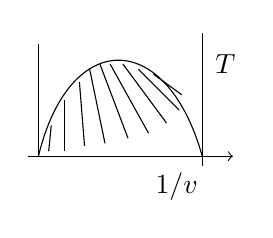
\begin{tikzpicture}[scale=0.65]
 \draw (-0.2,0)--(3.2,0);
 \draw[->] (3.2,0)--(3.8,0);
 \draw (0,0)--(0,2.2);
 \draw (3.2,-0.2)--(3.2,2.4);
 \draw (0,0).. controls (0.6,2.5) and (2.5,2.5)..(3.2,0);
 \draw (0.2,0.1)--(0.25,0.6);
 \draw (0.5,0.1)--(0.5,1.1);
 \draw (0.9,0.2)--(0.8,1.45);
 \draw (1.3,0.25)--(1,1.7);
 \draw (1.75,0.35)--(1.2,1.8);
 \draw (2.15,0.45)--(1.4,1.8);
 \draw (2.5,0.65)--(1.65,1.8);
 \draw (2.75,0.9)--(1.95,1.7);
 \draw (2.8,1.2)--(2.25,1.6);
 \node at (3.65,1.8) {$T$};
 \node at (2.7,-0.6) {$1/v$};
\end{tikzpicture}}}
[Dividing line.]

$S$ is a subcube. $S_\ell\subset V_\ell$.
$K_\ell$ is the side of $S_\ell$.
\begin{gather*}
 0<d<\frac{K_\ell}{\ell}<1-d.
\end{gather*}
Introduce a random variable.
$\mu(S_\ell)$ is the number of points of the arrangement $\theta$ that fall in $S_\ell$.
$\mu_{S_\ell}(\theta)$.
If
\begin{gather*}
 \mathsf{P}\left\{
 \left|\frac{\mu_{S_\ell}(\theta)}{K_\ell^\nu}-\frac1v\right|
 \right\}>\varepsilon\}\overset{/}{\longrightarrow}0,
 \qquad\varepsilon>0,
\end{gather*}
then there is a phase transition.
\Unclear{GELFAND-P000009}{probability-brace}{After the right absolute-value bar, the scan shows a brace before $>\varepsilon$ and another after $\varepsilon$. This inconsistent notation is retained; the usual event candidate has the absolute value greater than $\varepsilon$ inside a single pair of braces.}
[Beneath the first fraction:] density in the subcube.
[Beneath $1/v$:] density in the whole cube.
And a closely related condition is necessary.
(Physical meaning: coexistence of $2$ phases.)

\SourceFigure{GELFAND-P000009}{diagram-corner-cluster}{Original and existing typeset recreation.\par\smallskip\centering\resizebox{.93\linewidth}{!}{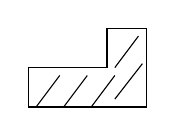
\begin{tikzpicture}[scale=0.5]
 \draw (0,0)--(3,0)--(3,2)--(2,2)--(2,1)--(0,1)--cycle;
 \draw (0.2,0)--(0.8,0.8);
 \draw (0.9,0)--(1.5,0.8);
 \draw (1.6,0)--(2.2,0.8);
 \draw (2.2,0.2)--(2.9,1.1);
 \draw (2.2,1)--(2.8,1.8);
\end{tikzpicture}}}
The boundary splits into components —
— but a connection through corners ($\nu=2$) or an edge ($\nu=3$)
is not counted.
\begin{gather*}
 \Gamma(\theta)=\sum_i\Gamma_i(\theta).
\end{gather*}
$\Gamma_i(\theta)$ is the length or area of a boundary component.
\underline{Definition.} Single out a special arrangement.
It depends on $3$ numbers, $N<\infty$, $D<\infty$, $\delta>0$.
\Unclear{GELFAND-P000009}{finite-parameter}{The first letter resembles $N$, but admits $M$; the enlarged fragment does not resolve the distinction. It is not automatically reconciled with the upper summation limit in the next frame.}
Number the cycles in decreasing order of length
\begin{gather*}
 \Gamma_1(\theta)\ge\Gamma_2(\theta)\ge\cdots .
\end{gather*}


\SourcePage{GELFAND-P000010}{unlabelled}
Conditions.
\begin{gather*}
 1)\quad\sum_{i=1}^{M}\Gamma_i(\theta)\le D\ell^{\nu-1}.
\end{gather*}
(Of the order of the surface of the large cube.)
\begin{gather*}
 2)\quad\sum_{i=M+1}^{\infty}
 \bigl(\Gamma_i(\theta)\bigr)^{\frac\nu{\nu-1}}
 \le\frac{\min(N_\ell,V_\ell-N_\ell)}{S_\nu}(1-\delta).
\end{gather*}
\Unclear{GELFAND-P000010}{small-cycles-sign}{The inequality sign before the fraction is heavily overwritten: candidates are $\le$ and $<$. The parameter in the upper limit of the first sum resembles $M$ or $N$.}
\begin{gather*}
 S_\nu\bigl(\Gamma_i(\theta)\bigr)^{\frac\nu{\nu-1}}
\end{gather*}
Area of a circle with length $\Gamma_i$.
A ball has maximal volume; this is an upper bound on the volume of the region inside the cycles.
(It is $<$ what is needed to contain all occupied points.)
([A word is cancelled; inserted above:] volume.
Inside small cycles $<$ the shaded area
and the white area.)
\Unclear{GELFAND-P000010}{small-volume-cancellation}{The word beneath the inserted ``volume'' is heavily cancelled and illegible. ``Area'' in the two lines is retained as in the scan, without replacing it with volume.}

\SourceFigure{GELFAND-P000010}{diagram-nested-cycles}{Four nested rounded boundaries: an outer shaded ring, a white gap and an inner ring with a white centre. Individual pen irregularities and merged strokes remain visible in the original.\par\smallskip\centering\resizebox{.93\linewidth}{!}{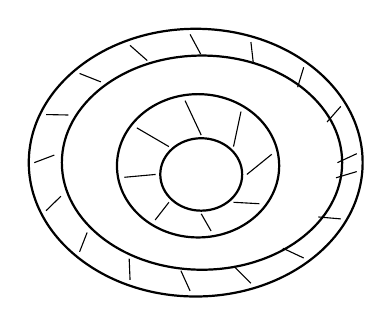
\begin{tikzpicture}[x=1cm,y=1cm]
\draw[thick](0,0)ellipse(2.12 and 1.7);\draw[thick](.08,0)ellipse(1.78 and 1.36);
\draw[thick](.03,-.04)ellipse(1.03 and .91);\draw[thick](.07,-.15)ellipse(.52 and .46);
\foreach \a in{0,22,...,352}{\draw({1.8*cos(\a)},{1.38*sin(\a)})--({2.05*cos(\a+4)},{1.63*sin(\a+4)});}
\foreach \a in{0,45,...,315}{\draw({.58*cos(\a)+.07},{.5*sin(\a)-.15})--({.95*cos(\a+10)+.03},{.84*sin(\a+10)-.04});}
\end{tikzpicture}}\par{\scriptsize Four boundaries and two shaded rings; schematic scale.}\par}
Neither all the points nor all the empty sites can be forced into it.
An example of an arrangement where the conditions do not hold.
\SourceFigure{GELFAND-P000010}{diagram-phase-mixture}{A rectangle is divided by an almost horizontal curve: three small rounded regions above, shading and several rounded unshaded regions below. The precise boundaries and number of lower regions are uncertain.\par\smallskip\centering\resizebox{.93\linewidth}{!}{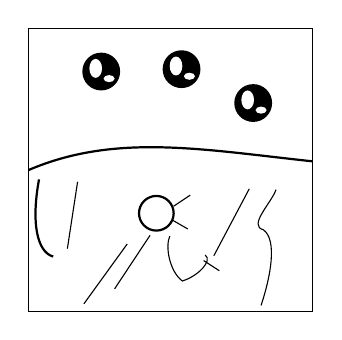
\begin{tikzpicture}[x=1cm,y=1cm]
\draw(0,0)rectangle(3.6,3.6);
\draw[thick](0,1.8)..controls(1.1,2.27)and(2.2,2.06)..(3.6,1.91);
\foreach \x/\y in{.92/3.05,1.94/3.08,2.85/2.65}{\fill(\x,\y)circle(.24);\fill[white](\x-.07,\y+.04)ellipse(.08 and .12);\fill[white](\x+.1,\y-.09)ellipse(.07 and .045);}
\draw[thick](1.62,1.25)circle(.22);
\draw(1.84,1.34)--(2.05,1.48);\draw(1.83,1.16)--(2.02,1.05);
\draw(1.79,.96)..controls(1.73,.82)and(1.79,.51)..(1.95,.39)..controls(2.15,.45)and(2.34,.65)..(2.24,.72);
\draw(2.22,.65)--(2.42,.52);
\draw[thick](.13,1.68)..controls(.03,1.14)and(.1,.76)..(.31,.7);
\draw(.62,1.65)--(.49,.8);\draw(.7,.1)--(1.25,.86);\draw(1.09,.29)--(1.54,.97);\draw(2.35,.71)--(2.8,1.56);\draw(2.95,.08)..controls(3.07,.44)and(3.16,.91)..(2.98,1.04)..controls(2.78,1.09)and(3.08,1.38)..(3.14,1.55);
\end{tikzpicture}}\par{\scriptsize Partial sketch: the uncertain lower contour remains open.}\par}
This is a phase transition.
Everything reduces to $2$ lemmas.

$1)$ $\exists M,D,\delta$ such that
the probability that the conditions hold $\longrightarrow1$,
if the stated condition holds.
[Beneath the parameters:] independent of everything.
\Unclear{GELFAND-P000010}{theorem-condition}{In the line after ``if ... holds'', the word looks like ``сформ.'' [stated] or ``строгое'' [strict]; nothing is supplied from the meaning.}

$2)$ \underline{Lemma $2$.}
If almost all arrangements are special, then there is a phase transition.
\underline{Idea of the proof of Lemma $2$.}
$G$ is the volume of the region enclosed by the small cycles.
\begin{gather*}
 G\le N_\ell(1-\delta),\qquad
 \frac{G}{V_\ell}\le\frac1v(1-\delta).
\end{gather*}
\SourceFigure{GELFAND-P000010}{diagram-grid}{A five-by-five rectangular grid; the second cell from the left in the fourth row from the top is emphasized. Caption: “Divided into subcubes”.\par\smallskip\centering\resizebox{.93\linewidth}{!}{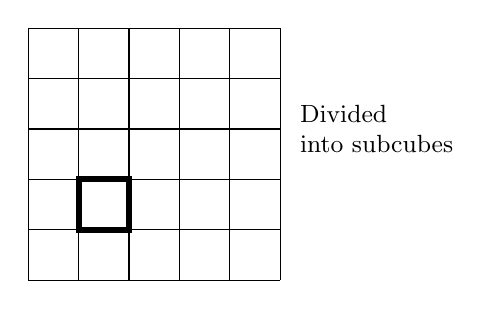
\begin{tikzpicture}[x=.64cm,y=.64cm]
\draw[step=1](0,0)grid(5,5);\draw[line width=2.2pt](1,1)rectangle(2,2);
\node[anchor=west,align=left,font=\small]at(5.2,3){\GridWords};
\end{tikzpicture}}\par{\scriptsize Five-by-five grid; cell (2,4) counted from left and top is emphasized.}\par}
There exists a subcube $S_\ell$:
\begin{gather*}
 \frac{G\cap S_\ell}{V_\ell}\le\frac1v(1-\delta).
\end{gather*}
\Unclear{GELFAND-P000010}{last-fraction}{In the numerator, the heavy sign before $\cap S_\ell$ resembles $G$; the denominator clearly resembles $V_\ell$. The candidate is retained; neither a measure of the intersection nor the subcube's volume is supplied from the meaning.}

\clearpage\section*{Full reading notes}
\subsection*{GELFAND-0001-U001}
\EvidenceBlock{GELFAND-P000001}{module-letter}{After “A is a ring” is a handwritten letter with a fork at the top and a lower hook; it recurs for the module and the ideal.}{Observation.}
\par\smallskip\noindent\textbf{Candidates: } \(\mathcal{J}\); \(\mathcal{I}\); J\par
\par\smallskip\noindent\textbf{Historical note: } A calligraphic J was used in the text as a graphical candidate; the notation was not identified from its mathematical meaning.\par
\par\smallskip\noindent\textbf{Fresh source comparison: } The same fork and lower hook are visible in three separate occurrences at 5×/10×. This supports a consistent graphical transcription but does not distinguish every possible conventional I/J letterform.\par
\subsection*{GELFAND-0001-U002}
\EvidenceBlock{GELFAND-P000001}{diagram-blowup}{In the upper half are three rounded contours with inner curves and two leftward arrows; D, D-prime, M and indices occur above and beside them.}{Observation.}
\par\smallskip\noindent\textbf{Candidates: } None proposed.\par
\par\smallskip\noindent\textbf{Historical note: } Uncertain inner curves and joins were not redrawn. The description and the source-figure entry retain a locator for comparison.\par
\par\smallskip\noindent\textbf{Fresh source comparison: } The complete diagram crop is now displayed at its typed description. Both leftward arrowheads are visible. A separate curved stroke rises from the lower contour toward the area beside D; its exact attachment to the upper contour is not asserted.\par
\subsection*{GELFAND-0001-U003}
\EvidenceBlock{GELFAND-P000001}{blowup-notation}{The upper index on \(M_0\) resembles H; over \(M_0\) at the lower region is a short stroke.}{Observation.}
\par\smallskip\noindent\textbf{Candidates: } \(M_0^H\); \(M'_0\); \(M_0^N\); \(M'_0\)\par
\par\smallskip\noindent\textbf{Historical note: } The indices and prime need comparison with the original.\par
\par\smallskip\noindent\textbf{Fresh source comparison: } Separate close crops show the dark upper index and the lower prime at the reading itself. The lower prime is distinct; the dark upper sign still does not justify excluding N in favor of H.\par
\subsection*{GELFAND-0001-U006}
\EvidenceBlock{GELFAND-P000001}{origin-example}{To the right of the \(R^2\) example the line begins with a joined group of letters and ends “into 0, a projective line”.}{Observation.}
\par\smallskip\noindent\textbf{Candidates: } Вклеив. в 0 проект. прямой [Gluing a projective line into 0]; Оклеив. в 0 проект. прямой [alternative initial abbreviation]\par
\par\smallskip\noindent\textbf{Historical note: } The phrase is given inside the uncertain-reading entry, without choosing from the mathematical meaning of a blow-up.\par
\par\smallskip\noindent\textbf{Fresh source comparison: } The wider context and 5×/10× details strongly favor the initial В and the abbreviation Вклеив. The historical alternative remains visible; the source wording is not replaced by a standard construction of a blow-up.\par

\subsection*{GELFAND-0001-U007}
\EvidenceBlock{GELFAND-P000002}{ideal-selection}{A rereading of the enlarged original fragment favors “polynomials, starting with degree 1”; the middle strokes of the abbreviation нач. are still not fully distinguishable.}{Observation.}
\par\smallskip\noindent\textbf{Candidates: } мн., нач. с 1-й степени [polynomials, starting with degree 1]; мн., к-ст. с 1-й степенью [alternative abbreviation; expansion uncertain]\par
\par\smallskip\noindent\textbf{Historical note: } The first candidate was selected from the shape of the original line; it was not replaced by the standard definition of Proj.\par
\par\smallskip\noindent\textbf{Fresh source comparison: } The line ending is visible in the wider crop and separate 5×/10× details. Its first abbreviation Выбр. is visible too, but its expansion could express selecting or discarding. The English text retains that abbreviation rather than deciding the operation from the construction. The strokes favor нач. at the end; the historical alternative remains recorded.\par

\subsection*{GELFAND-0001-U008}
\EvidenceBlock{GELFAND-P000002}{open-set-notation}{In a separate rereading, the first letter after “then” matches the shape of \(O_X\) above; the second matches the ideal letter with a lower hook.}{Observation.}
\par\smallskip\noindent\textbf{Candidates: } \(O_U,J_U\); \(O_U,I_U\)\par
\par\smallskip\noindent\textbf{Historical note: } The initial reading of the first letter as J was corrected from the scan. The possible I/J distinction in the second letter remains, independently of the standard sheaf construction.\par
\par\smallskip\noindent\textbf{Fresh source comparison: } The corrected context now includes the whole lower subscripts. The rounded first sign and forked, hooked second sign match the earlier pair. These shapes support O followed by the ideal letter, without deciding every conventional I/J distinction. Separate 5×/10× details were inspected.\par

\subsection*{GELFAND-0001-U009}
\EvidenceBlock{GELFAND-P000002}{fractions-sentence}{After “ring of fractions” one can see “numer., denom., not belonging to any of the ideals”, but the abbreviation boundaries and the scope of the last phrase are unclear.}{Observation.}
\par\smallskip\noindent\textbf{Candidates: } числ., знамен., не прин. ни одному из идеалов [numer., denom., not belonging to any of the ideals]; числ.; знамен. не прин. ни одному из идеалов [numer.; denom. not belonging to any of the ideals]\par
\par\smallskip\noindent\textbf{Historical note: } The punctuation was not corrected from the definition of localization.\par
\par\smallskip\noindent\textbf{Fresh source comparison: } Four overlapping source parts retain the line ending числ., the following знамен., and the phrase about the ideals. The abbreviations are visible at 5×/10×; their punctuation does not establish which nouns the restriction modifies. No missing qualifier is supplied.\par

\subsection*{GELFAND-0001-U010}
\EvidenceBlock{GELFAND-P000002}{margin-grothendieck}{The right-hand note beside two vertical arrows reads “Grothendieck — blow up …”; the final word is written continuously.}{Observation.}
\par\smallskip\noindent\textbf{Candidates: } идеально [ideally]; идеалы [ideals]\par
\par\smallskip\noindent\textbf{Historical note: } The final word is not asserted.\par
\par\smallskip\noindent\textbf{Fresh source comparison: } The wider crop includes both downward arrows and the full note. The joined final strokes favor идеально, but do not securely exclude идеалы. The literal candidate “blow up ideally” is retained with the alternative; the wording is not regularized into a definition.\par

\subsection*{GELFAND-0001-U011}
\EvidenceBlock{GELFAND-P000002}{quadratic-coefficients}{After J tensor J is a thick two-sided mark and a quadratic polynomial; the coefficients resemble \(a_2\), \(2b_2\), c.}{Observation.}
\par\smallskip\noindent\textbf{Candidates: } \(a_2x^2+2b_2xy+cy^2+\cdots\); \(a_2x^2+2b_2xy+c_2y^2+\cdots\)\par
\par\smallskip\noindent\textbf{Historical note: } The index on the final coefficient and the direction of the thick mark are uncertain.\par
\par\smallskip\noindent\textbf{Fresh source comparison: } The complete context and separate details show \(a_2\) and \(2b_2\). A small upper stroke is visible near the c-shaped coefficient; it is not a secure lower index 2. The thick connecting mark is retained as an uncertain graphical candidate, without inferring an isomorphism.\par

\subsection*{GELFAND-0001-U012}
\EvidenceBlock{GELFAND-P000002}{last-sign}{At the lower edge is \(a_0+(a_1x-b_1y)z+\cdots\); the horizontal sign before \(b_1y\) looks like a minus.}{Observation.}
\par\smallskip\noindent\textbf{Candidates: } \(a_0+(a_1x-b_1y)z+\cdots\); \(a_0+(a_1x+b_1y)z+\cdots\)\par
\par\smallskip\noindent\textbf{Historical note: } The visible minus is retained in the body; the next scan has a plus. The arrow at left is written heavily.\par
\par\smallskip\noindent\textbf{Fresh source comparison: } The enlarged sign is a horizontal minus; no vertical crossing stroke is visible. The next source page has a plus. Both source readings remain, and the mathematical commentary does not use a change of sign to alter either transcription. The heavy arrow still has uncertain direction.\par

\subsection*{GELFAND-0001-U013}
\EvidenceBlock{GELFAND-P000003}{directions}{In parentheses after “plane” is the abbreviation “замк. всеми возм. напр.” and a sign resembling sigma before “process”.}{Observation.}
\par\smallskip\noindent\textbf{Candidates: } замк. всеми возм. напр. — σ-процесс [first abbreviation uncertain; with all possible directions — sigma-process]; зам. всеми возм. напр. — σ-процесс [alternative first abbreviation; with all possible directions — sigma-process]\par
\par\smallskip\noindent\textbf{Historical note: } The abbreviations were not expanded or replaced by a term inferred from the meaning.\par
\par\smallskip\noindent\textbf{Fresh source comparison: } The initial abbreviation and the sigma-like sign have been inspected at 5×/10×. The final short stroke of the first abbreviation is still not secure. The translation expands the readily legible neighboring abbreviations, but keeps замк. itself visibly unexpanded.\par

\subsection*{GELFAND-0001-U014}
\EvidenceBlock{GELFAND-P000003}{cross-cancellation}{Between “In the space” and the cross is a heavily cancelled short group of letters.}{Observation.}
\par\smallskip\noindent\textbf{Candidates: } None proposed.\par
\par\smallskip\noindent\textbf{Historical note: } The cancellation itself is marked; the underlying text cannot be read confidently.\par
\par\smallskip\noindent\textbf{Fresh source comparison: } The opaque horizontal cancellation remains unreadable even at 10×. The separate original cross is also shown beside the existing two-stroke native recreation. Its thick ends do not establish intentional arrowheads; the recreation retains two crossing, unarrowed strokes.\par

\subsection*{GELFAND-0001-U016}
\EvidenceBlock{GELFAND-P000003}{ising-cancellation}{Under the name Dobrushin, before “Find”, a group of letters is completely crossed out.}{Observation.}
\par\smallskip\noindent\textbf{Candidates: } None proposed.\par
\par\smallskip\noindent\textbf{Historical note: } The visible cancellation is preserved; the original word was not reconstructed.\par
\par\smallskip\noindent\textbf{Fresh source comparison: } The wider context identifies the position before “Find”; the 5×/10× details show multiple dense crossing strokes. They do not support a complete word, so no candidate is invented.\par

\subsection*{GELFAND-0001-U017}
\EvidenceBlock{GELFAND-P000003}{configuration-letter}{Before \((x_1,\ldots,x_N)\), and later in the formulas, is a sign with a rounded lower part and a dark upper stroke.}{Observation.}
\par\smallskip\noindent\textbf{Candidates: } \(\theta\); \(b\); в\par
\par\smallskip\noindent\textbf{Historical note: } The fragment uses theta as a single graphical candidate for this recurring sign.\par
\par\smallskip\noindent\textbf{Fresh source comparison: } The corrected crop includes the entire left-hand sign and its equality. Two separate occurrences were inspected at 5×/10×. The divided loop and thick upper stroke are consistent, but do not securely exclude b or Cyrillic в. The theta transcription remains explicitly provisional.\par

\subsection*{GELFAND-0001-U018}
\EvidenceBlock{GELFAND-P000003}{energy-cancellation}{Between “The Ising model” and \(U(\theta)\) is a separate completely inked-out sign.}{Observation.}
\par\smallskip\noindent\textbf{Candidates: } None proposed.\par
\par\smallskip\noindent\textbf{Historical note: } The cancelled sign was not taken as a mathematical operator.\par
\par\smallskip\noindent\textbf{Fresh source comparison: } The sign remains opaque at 5×/10×; its dark mass and the underlying strokes do not identify an operator or letter. Its location and cancellation are preserved, without assigning it a mathematical role.\par

\subsection*{GELFAND-0001-U019}
\EvidenceBlock{GELFAND-P000003}{energy-case}{In the second branch of u=..., the sign before \((x_i,x_j)=1\) resembles rho; the caption below begins \(u(\theta)\).}{Observation.}
\par\smallskip\noindent\textbf{Candidates: } \(\rho(x_i,x_j)=1\); \(\chi(x_i,x_j)=1\)\par
\par\smallskip\noindent\textbf{Historical note: } A sign resembling a semicolon is visible after the unit value. The small u in the caption was not replaced with U.\par
\par\smallskip\noindent\textbf{Fresh source comparison: } A corrected context contains the complete equality, and a repaired 5×/10× target shows the rho-shaped letter itself. The earlier narrow detail missed that target and is not used as evidence for it. The full lower caption clearly begins with a small u-shaped letter. The branch punctuation and the U/u difference remain diplomatic; their mathematical implications are discussed separately.\par

\subsection*{GELFAND-0001-U020}
\EvidenceBlock{GELFAND-P000003}{partition-domain}{The first normalizing quantity looks like \(Z(V_\ell,N)\); below is \(Z(\ell,N)\). The set under the second sum has the shape of a handwritten B.}{Observation.}
\par\smallskip\noindent\textbf{Candidates: } \(Z(V_\ell,N);\ Z(\ell,N);\ \theta\in B\); \(Z(V_\ell,N);\ Z(\ell,N);\ \theta\in\mathcal B\)\par
\par\smallskip\noindent\textbf{Historical note: } The difference in arguments is preserved. The set symbol was not identified with the event B from its meaning.\par
\par\smallskip\noindent\textbf{Fresh source comparison: } Separate 5×/10× details confirm the visible \(V_\ell\) in the first denominator and ell in the next line. The set under the second sum carries an added upper stroke, supporting a distinct graphical candidate, but ordinary B versus a calligraphic form remains uncertain. The transcription keeps the event and configuration-set candidates distinct.\par

\subsection*{GELFAND-0001-U021}
\EvidenceBlock{GELFAND-P000003}{attraction-note}{After “The molecules attract” are parentheses with inked signs, arrows, and the words “neighbors” and “probab.”.}{Observation.}
\par\smallskip\noindent\textbf{Candidates: } соседи > их вероятн. [neighbors > their probab.]; соседи > его вероятн. [neighbors > its probab.]\par
\par\smallskip\noindent\textbf{Historical note: } The provisional caption was given only as a candidate; the drawing was not converted into a precise assertion.\par
\par\smallskip\noindent\textbf{Fresh source comparison: } The filled marks, arrows and caption are displayed together. At 5×/10× the pronoun looks closer to его than to их, but the elliptical phrase still does not support a complete assertion. The inherited body candidate remains visibly marked as uncertain and both historical alternatives are retained.\par

\subsection*{GELFAND-0001-U022}
\EvidenceBlock{GELFAND-P000003}{density-cancellation}{Before \(V_\ell/N_\ell\) is a heavily cancelled short mark.}{Observation.}
\par\smallskip\noindent\textbf{Candidates: } None proposed.\par
\par\smallskip\noindent\textbf{Historical note: } The original sign was not recovered.\par
\par\smallskip\noindent\textbf{Fresh source comparison: } The cancelled mark remains unreadable in the enlarged details. The wider source fragment includes the fraction and \(v=\mathrm{const}\), so its place is inspectable. The written ratio \(V_\ell/N_\ell\) is retained, rather than silently changed to particle density \(N_\ell/V_\ell\).\par


\subsection*{GELFAND-0001-U024}
\EvidenceBlock{GELFAND-P000004}{pressure-letter}{The first argument of \(p(\cdot,T)\) is heavily written. The fraction contains \(\partial f/\partial v\) and is preceded by T; no minus is visible before the derivative.}{Observation.}
\par\smallskip\noindent\textbf{Candidates: } \(p(v,T)=T\partial f/\partial v\); \(p(\nu,T)=T\partial f/\partial v\)\par
\par\smallskip\noindent\textbf{Historical note: } No thermodynamically expected correction of the sign was substituted.\par
\par\smallskip\noindent\textbf{Fresh source comparison: } The whole frame and 3×/5×/10× details show no minus before T. The first argument remains a heavily written v-like sign; \(\nu\) is not excluded. A separate commentary derives a possible plus under an explicit definition of f; this does not settle the letter or amend the source.\par

\subsection*{GELFAND-0001-U025}
\EvidenceBlock{GELFAND-P000004}{diagram-phase-point}{The upper right drawing has a rising curve with a flat middle, an arrow toward it, and the caption “points of phase transition” [точки фаз. перехода].}{Observation.}
\par\smallskip\noindent\textbf{Candidates: } None proposed.\par
\par\smallskip\noindent\textbf{Historical note: } The precise axes, points, and shape of the transitions are not identified confidently.\par
\par\smallskip\noindent\textbf{Fresh source comparison: } After extending the crop downward, the whole caption “точки фаз. перехода” is visible, in the plural. No axes are visible. The typeset sketch represents the flat middle, point, and curved pointer; it does not assert the precise direction of the heavily inked arrowhead.\par

\subsection*{GELFAND-0001-U026}
\EvidenceBlock{GELFAND-P000004}{diagram-cancelled-graph}{At left are two axes, with 0 and \(\infty\) by the horizontal axis; several heavily overwritten curves and straight lines, and a vertical letter.}{Observation.}
\par\smallskip\noindent\textbf{Candidates: } vertical label \(\varphi\); vertical label f\par
\par\smallskip\noindent\textbf{Historical note: } The crossed-out lines were retained by description; no precise underlying curve was selected.\par
\par\smallskip\noindent\textbf{Fresh source comparison: } Even at 10×, individual connections of the underlying curves cannot be separated from the heavy cancellations. The partial typeset sketch shows only the secure axes, 0 and \(\infty\); the disputed vertical letter remains among the candidates. The neighboring clean graph at right is a different drawing and is shown separately.\par

\subsection*{GELFAND-0001-U028}
\EvidenceBlock{GELFAND-P000004}{diagram-onsager}{Axes T and v; a curve with a vertex, a vertical through the vertex, \(1/2\) below, and a small wavy branch at right.}{Observation.}
\par\smallskip\noindent\textbf{Candidates: } None proposed.\par
\par\smallskip\noindent\textbf{Historical note: } The branches and their connections require the original drawing; an exact redrawing had not been made.\par
\par\smallskip\noindent\textbf{Fresh source comparison: } The left branch has an additional stroke; the vertical passes through the vertex, with \(1/2\) below. A small visible gap separates the short wavy line at right from the vertex. The typeset sketch retains that gap without assigning physical meaning to the line.\par

\subsection*{GELFAND-0001-U029}
\EvidenceBlock{GELFAND-P000004}{kac-helfand-note}{A repeated twofold enlargement of the line beneath Kac, Helfand shows “точн. в яв. виду для нек-рых случаях” [exact, in explicit form, for some cases]; the word endings are not completely clear.}{Observation.}
\par\smallskip\noindent\textbf{Candidates: } точн. в яв. виду для нек-рых случаях [literal source endings]; точн. в яв. виде для нек-рых случаев [alternative endings]\par
\par\smallskip\noindent\textbf{Historical note: } The word случая... [case...] has now been read, replacing the erroneous initial сущ.; neither grammar nor the known result is used to correct the ending silently.\par
\par\smallskip\noindent\textbf{Fresh source comparison: } The wide crop retains the names and the entire line. The 5×/10× details favor виду and случаях. The historical alternatives виде and случаев remain in full; the English body conveys the meaning while separately displaying the nonstandard source endings.\par

\subsection*{GELFAND-0001-U030}
\EvidenceBlock{GELFAND-P000004}{diagram-subcube}{A large square and a smaller outlined region, H at the center and h above; the small contour has overlapping rounded and straight strokes.}{Observation.}
\par\smallskip\noindent\textbf{Candidates: } None proposed.\par
\par\smallskip\noindent\textbf{Historical note: } The source was retained as a drawing, without selecting an exact boundary from the term “subcube”.\par
\par\smallskip\noindent\textbf{Fresh source comparison: } Both straight and rounded strokes of the inner boundary are visible at 5×/10×; h above H is readable. The outer lines have gaps. The typeset sketch retains the overlap and gaps rather than replacing the drawing with a perfect square or circle.\par

\subsection*{GELFAND-0001-U031}
\EvidenceBlock{GELFAND-P000004}{probability-bar}{A vertical bar is visible before \(>\varepsilon\); before the first fraction, a possible left bar merges with the brace.}{Observation.}
\par\smallskip\noindent\textbf{Candidates: } \(\mathsf P\{\mu_H/h^\nu-1/v\mid>\varepsilon\}\to0\); \(\mathsf P\{|\mu_H/h^\nu-1/v|>\varepsilon\}\to0\)\par
\par\smallskip\noindent\textbf{Historical note: } The matching bar was not added silently; the visible candidate was left in the body.\par
\par\smallskip\noindent\textbf{Fresh source comparison: } The right vertical stroke is separate from \(>\varepsilon\). An independent left absolute-value bar beside the opening brace cannot be established even at 10×. The next frame clearly has paired bars, but that comparison does not change this frame’s notation.\par

\subsection*{GELFAND-0001-U032}
\EvidenceBlock{GELFAND-P000004}{bottom-mark}{At the lower right edge, a small isolated sign resembles 2 or a fragment of a letter.}{Observation.}
\par\smallskip\noindent\textbf{Candidates: } 2; fragment of a letter\par
\par\smallskip\noindent\textbf{Historical note: } No confident page number was assigned.\par
\par\smallskip\noindent\textbf{Fresh source comparison: } At 5×/10×, only a short hook and fragmentary edge strokes remain. The digit 2 and a fragment of a letter remain candidates; no number is assigned.\par

\subsection*{GELFAND-0001-U033}
\EvidenceBlock{GELFAND-P000004}{margin-left}{At the extreme left edge of the frame, a narrow strip of neighboring text is cut off to isolated endings and strokes; a separate crop at native pixel resolution was checked.}{Observation.}
\par\smallskip\noindent\textbf{Candidates: } None proposed.\par
\par\smallskip\noindent\textbf{Historical note: } Connected text is unavailable in this frame; the page has unreadable status because of this portion. The main writing surface has been read and transcribed.\par
\par\smallskip\noindent\textbf{Fresh source comparison: } Four overlapping source strips retain the entire available left edge. It is already clipped in the whole original frame; further magnification cannot restore the missing portions of letters. No independently readable words were established.\par

\subsection*{GELFAND-0001-U034}
\EvidenceBlock{GELFAND-P000005}{exponential-rate}{In \(O(e^{\cdots\beta})\), the sign between the minus and \(\beta\) is heavily obscured; before the preceding phrase is an opening round parenthesis without a clearly visible closing parenthesis.}{Observation.}
\par\smallskip\noindent\textbf{Candidates: } \(O(e^{-N\beta})\); \(O(e^{-\ell\beta})\)\par
\par\smallskip\noindent\textbf{Historical note: } The obscured sign was not declared settled, and a missing parenthesis was not added to the source text.\par
\par\smallskip\noindent\textbf{Fresh source comparison: } The corrected crop includes the tops of all overlapping strokes in the exponent. The minus and \(\beta\) are visible; the intervening sign cannot reliably be distinguished as N or \(\ell\) at 10×. Separate crops show the insertion “absence” and the opening parenthesis. The insertion is retained explicitly, and the parenthesis is not closed editorially.\par

\subsection*{GELFAND-0001-U035}
\EvidenceBlock{GELFAND-P000005}{complement-label}{In the line about \(\theta_2\) and \(N-k\) particles, a short upper stroke is visible by H.}{Observation.}
\par\smallskip\noindent\textbf{Candidates: } \(\overline H\); \(H\)\par
\par\smallskip\noindent\textbf{Historical note: } The barred candidate was used in the text; the complement was not determined solely from its meaning.\par
\par\smallskip\noindent\textbf{Fresh source comparison: } The wider crop shows both H labels and the horizontal stroke between them. It may be an overbar on the lower H or an underline on the upper H; the 5×/10× details do not settle its attachment. The historical barred candidate remains a candidate, not an established reading.\par

\subsection*{GELFAND-0001-U036}
\EvidenceBlock{GELFAND-P000005}{boundary-exponent}{After the words about the number of boundary points, the exponent of V is tightly written: \(\nu\)-1, a slanted fraction stroke, and \(\nu\).}{Observation.}
\par\smallskip\noindent\textbf{Candidates: } \(V^{\nu-1/\nu}\); \(V^{(\nu-1)/\nu}\)\par
\par\smallskip\noindent\textbf{Historical note: } The first candidate was retained. In the following bound involving N, the exponent is written more clearly as a fraction.\par
\par\smallskip\noindent\textbf{Fresh source comparison: } The two crops show the tight exponent on V and the explicit common fraction \((\nu-1)/\nu\) on N. Their difference is retained. A separate mathematical commentary derives boundary scaling for an explicitly defined lattice model; this derivation is not substituted for reading the ink.\par

\subsection*{GELFAND-0001-U037}
\EvidenceBlock{GELFAND-P000005}{theta-factor}{In the factor \(\exp\{\cdots N^{2/3}\}\), the letter resembles \(\theta\); below it, the same letter is explained as “bounded parameter” [огранич. параметр].}{Observation.}
\par\smallskip\noindent\textbf{Candidates: } \(\theta\); \(\Theta\)\par
\par\smallskip\noindent\textbf{Historical note: } It may differ from the configuration symbol; their identity has not been declared proved.\par
\par\smallskip\noindent\textbf{Fresh source comparison: } Both factors and the caption show an oval sign with a transverse stroke. The \(\theta/\Theta\) case and its distinction from the configuration symbol remain unsettled. The exponent \(2/3\) is clearly visible; it is not replaced by the general exponent written above.\par

\subsection*{GELFAND-0001-U073}
\EvidenceBlock{GELFAND-P000005}{physical-meaning-heading}{The first explanatory line after the phase-transition condition begins with an abbreviation best read as “Нагл. смысл.” [Нагл. meaning]; its middle strokes merge.}{Observation.}
\par\smallskip\noindent\textbf{Candidates: } Нагл. смысл. [Нагл. meaning]; Нач. смысл. [Нач. meaning]\par
\par\smallskip\noindent\textbf{Historical note: } The abbreviation was not expanded into a complete word; the candidate was selected from the original fragment at 3× magnification.\par
\par\smallskip\noindent\textbf{Fresh source comparison: } The whole word and 5×/10× details favor Нагл. The alternative Нач. and the historical uncertainty about the middle strokes remain recorded; no full word is supplied.\par

\subsection*{GELFAND-0001-U039}
\EvidenceBlock{GELFAND-P000006}{subcube-power}{In the argument of f, a visible exponent 3 stands above h; the following line also has \(\ell\)\textasciicircum{}3-h\textasciicircum{}3.}{Observation.}
\par\smallskip\noindent\textbf{Candidates: } \(h^3/k;\ (\ell^3-h^3)/(N-k)\); \(h^\nu/k;\ (\ell^\nu-h^\nu)/(N-k)\)\par
\par\smallskip\noindent\textbf{Historical note: } The visible 3 was retained, without standardizing it to the dimension symbol \(\nu\) on neighboring lines.\par
\par\smallskip\noindent\textbf{Fresh source comparison: } The whole frame, both contexts and 5×/10× details support 3 on h and \(\ell\). The readings h\textasciicircum{}3 and \(\ell\)\textasciicircum{}3-h\textasciicircum{}3 have graphical support; neighboring \(\nu\) does not justify replacing them. The historical alternatives remain recorded.\par

\subsection*{GELFAND-0001-U040}
\EvidenceBlock{GELFAND-P000006}{limit-notation}{The probability argument has \(\mu\)\_H=k followed by a rounded sign; at right are a density sign and two branches with zeros. Text above the second branch is inked over.}{Observation.}
\par\smallskip\noindent\textbf{Candidates: } \(\mu_H=k\rho;\ \rho=1/v\); \(\mu_H=k\theta;\ \rho=1/v\); \(\mu_H=k\delta;\ \delta=1/v\)\par
\par\smallskip\noindent\textbf{Historical note: } The inked-over text is unreadable. The two visible zeros were not replaced by different limits according to an expected meaning.\par
\par\smallskip\noindent\textbf{Fresh source comparison: } The rounded letter after k has a curved descending stem, supporting \(\rho\); \(\theta\) and \(\delta\) remain historical alternatives. Both zeros are retained. The inked-over writing above the second branch remains unreadable at 10×. The small step-like drawing is shown separately.\par

\subsection*{GELFAND-0001-U041}
\EvidenceBlock{GELFAND-P000006}{diagram-cell-clusters}{Inside a large square frame, a vertical chain of shaded cells is at left, and an angular group of cells at right.}{Observation.}
\par\smallskip\noindent\textbf{Candidates: } None proposed.\par
\par\smallskip\noindent\textbf{Historical note: } The exact cell count and internal marks are uncertain; the original drawing is required.\par
\par\smallskip\noindent\textbf{Fresh source comparison: } Comparing the rendered page with the 10× details does not securely distinguish the left chain’s internal divisions from its dense hatching. The provisional new count of three cells was overconfident and was withdrawn before publication. At right, three cells form a corner. The partial typeset sketch at left shows only its outer outline and hatching; the cell count remains unresolved. The original remains alongside.\par

\subsection*{GELFAND-0001-U042}
\EvidenceBlock{GELFAND-P000006}{gamma-prime}{In the two exponentials after the equality, a \(\Gamma\)-like sign has a possible prime at its upper right.}{Observation.}
\par\smallskip\noindent\textbf{Candidates: } \(\Gamma^{\prime}(\theta)\); \(\Gamma(\theta)\)\par
\par\smallskip\noindent\textbf{Historical note: } The primed candidate was used in the body despite the visible caption referring to length/area.\par
\par\smallskip\noindent\textbf{Fresh source comparison: } The corrected r3 details favor \(\Gamma\) without a separate prime in both places; strokes overlap near the lower parenthesis. The initial r2 details clipped the tops and do not decide the prime. Both alternatives and the historical body candidate remain; the definition of length does not substitute for reading the ink.\par

\subsection*{GELFAND-0001-U043}
\EvidenceBlock{GELFAND-P000006}{energy-bound}{The bottom formula begins -U(\(\theta\)), followed by an overwritten sign before \(\Sigma\)(2\(\nu\)-\(\delta\)), then 2\(\nu\)N and a sum of \(\delta\) with lower index \(\Gamma\)'(\(\theta\)).}{Observation.}
\par\smallskip\noindent\textbf{Candidates: } \(-U(\theta)\ge\sum(2\nu-\delta)=2\nu N-\sum_{\Gamma^{\prime}(\theta)}\delta\)\par\smallskip\(-U(\theta)\le\sum(2\nu-\delta)=2\nu N-\sum_{\Gamma^{\prime}(\theta)}\delta\)\par\smallskip\(-U(\theta)=\sum(2\nu-\delta)=2\nu N-\sum_{\Gamma^{\prime}(\theta)}\delta\)\par
\par\smallskip\noindent\textbf{Historical note: } The energy normalization was not corrected to the standard model; the index and final sign also require checking.\par
\par\smallskip\noindent\textbf{Fresh source comparison: } At 10× the crossed strokes before the sum do not uniquely determine \(\ge\), \(\le\) or =. The last sum’s lower index is heavily written over. A separate edge count checks a possible factor of two under explicit conventions and does not amend this line.\par

\subsection*{GELFAND-0001-U044}
\EvidenceBlock{GELFAND-P000007}{diagram-small-clusters}{A small square frame at right contains two densely filled rounded patches and several strokes in its upper left corner.}{Observation.}
\par\smallskip\noindent\textbf{Candidates: } None proposed.\par
\par\smallskip\noindent\textbf{Historical note: } The small strokes and inked-in internal contours cannot be enumerated confidently.\par
\par\smallskip\noindent\textbf{Fresh source comparison: } The two large patches and their white openings are distinguishable. Several short strokes at upper left stand above a curved lower stroke; they are not assigned a definite particle count or letter reading. A partial typeset recreation preserves the arrangement and the uncertainty of those marks.\par

\subsection*{GELFAND-0001-U045}
\EvidenceBlock{GELFAND-P000007}{diagram-cycles}{A large frame at left contains three separate rounded groups with internal contours and hatching; one contains a central island.}{Observation.}
\par\smallskip\noindent\textbf{Candidates: } None proposed.\par
\par\smallskip\noindent\textbf{Historical note: } The nested cycles and hatching were not replaced by an approximately invented figure.\par
\par\smallskip\noindent\textbf{Fresh source comparison: } The full context and new details distinguish an upper-left horseshoe with a white gap open below, a right-hand ring, and a lower-left group with a central island. The typeset sketch preserves that nesting and open gap. It does not claim to recover every pen irregularity or hatch endpoint.\par

\subsection*{GELFAND-0001-U046}
\EvidenceBlock{GELFAND-P000007}{special-arrangement-count}{After \(\exists\), the first finite parameter resembles N; the summation limit in condition 1 resembles M.}{Observation.}
\par\smallskip\noindent\textbf{Candidates: } \(\exists N<\infty,\ D<\infty,\ \delta>0;\ \sum^{M}\); \(\exists M<\infty,\ D<\infty,\ \delta>0;\ \sum^{M}\)\par
\par\smallskip\noindent\textbf{Historical note: } The difference between the letters was not removed on the basis of the repeated definition in later scans.\par
\par\smallskip\noindent\textbf{Fresh source comparison: } In the full context the first letter still favors N, while the later limit favors M. The small r2 detail shows only <\(\infty\) and cannot by itself decide the letter. The difference is not reconciled with the subsequent definition.\par

\subsection*{GELFAND-0001-U047}
\EvidenceBlock{GELFAND-P000007}{large-cycles-power}{The exponent on the length in the first condition has a small fraction bar: \(\nu\)-1 above \(\nu\).}{Observation.}
\par\smallskip\noindent\textbf{Candidates: } \(\ell^{(\nu-1)/\nu}\); \(\ell^{\nu-1}\)\par
\par\smallskip\noindent\textbf{Historical note: } The fractional candidate was retained. GELFAND-P000010 visibly has exponent \(\nu\)-1; it was not imported here.\par
\par\smallskip\noindent\textbf{Fresh source comparison: } The 5×/10× details clearly show the fraction bar and a separate \(\nu\) below it, supporting (\(\nu\)-1)/\(\nu\). The historical alternative and the difference from frame 10 remain recorded; the expected surface exponent does not alter the ink.\par

\subsection*{GELFAND-0001-U048}
\EvidenceBlock{GELFAND-P000007}{small-cycles-sum}{The second sum visibly has upper M and lower i=1; its caption says “all the others small”, and no continuation follows the power.}{Observation.}
\par\smallskip\noindent\textbf{Candidates: } \(\sum_{i=1}^{M}\Gamma_i^{\nu/(\nu-1)}\); \(\sum_{i=M+1}^{\infty}\Gamma_i^{\nu/(\nu-1)}\)\par
\par\smallskip\noindent\textbf{Historical note: } Only the visible limits were put into the body; no condition was added from a later scan.\par
\par\smallskip\noindent\textbf{Fresh source comparison: } The context preserves the upper letter and caption; 5×/10× details confirm lower i=1. No continuation follows the expression before the dividing line. The sum starting at i=M+1 and the bound in frame 10 are not substituted.\par

\subsection*{GELFAND-0001-U050}
\EvidenceBlock{GELFAND-P000007}{field-margin}{At right of the equation are several lines and an arrow near \(\varphi\) and C\_0\textasciicircum{}\(\infty\); the upper part resembles “б, ф-й на”.}{Observation.}
\par\smallskip\noindent\textbf{Candidates: } б, ф-й на C\_0\textasciicircum{}\(\infty\) [fragment: functions on C\_0\textasciicircum{}\(\infty\)]; об. ф-й на C\_0\textasciicircum{}\(\infty\) [source abbreviation: functions on C\_0\textasciicircum{}\(\infty\)]\par
\par\smallskip\noindent\textbf{Historical note: } The text was not expanded into a definition of a distribution on semantic grounds.\par
\par\smallskip\noindent\textbf{Fresh source comparison: } The enlarged initial sign admits “об.”, but overlapping strokes do not securely expand the abbreviation. C\_0\textasciicircum{}\(\infty\) and the arrow are distinguishable. The separate “\(\varphi\) — мн.” also remains abbreviated. No definition of a generalized function is inserted from context.\par

\subsection*{GELFAND-0001-U051}
\EvidenceBlock{GELFAND-P000007}{ideal-signature}{In “Take the ideal, generated by (F\_: f\(\in\)C\_0\textasciicircum{}\(\infty\))”, the sign after the dash resembles \(\Omega\); the index on F is densely written.}{Observation.}
\par\smallskip\noindent\textbf{Candidates: } \(F_f;\ \Omega\); \(F_j;\ \Omega\); \(F_f;\ J\)\par
\par\smallskip\noindent\textbf{Historical note: } The symbols remain candidates and were not corrected through the algebraic construction.\par
\par\smallskip\noindent\textbf{Fresh source comparison: } The corrected context extends rightward through \(\Omega\). The sign after the dash resembles a broad \(\Omega\) with lower ends. The F index merges with neighboring strokes, so f remains a preference rather than an established reading. Algebra does not decide the letters.\par

\subsection*{GELFAND-0001-U052}
\EvidenceBlock{GELFAND-P000007}{evaluation-target}{After “a homomorphism into”, a rounded letter with a vertical stroke resembles \(\Phi\).}{Observation.}
\par\smallskip\noindent\textbf{Candidates: } \(\Phi\); a field denoted by a similar-looking letter\par
\par\smallskip\noindent\textbf{Historical note: } It was not automatically replaced by a number field.\par
\par\smallskip\noindent\textbf{Fresh source comparison: } At 5×/10× two rounded parts and a vertical stem support \(\Phi\) graphically. A field is not supplied in the diplomatic line. The separate evaluation-map commentary states its own assumptions and does not correct the source notation.\par

\subsection*{GELFAND-0001-U053}
\EvidenceBlock{GELFAND-P000008}{algebra-ring-letter}{Above p in the fraction is a dark letter with an upper horizontal and a rounded part; the similar letter in the caption at right is followed by “all equations”.}{Observation.}
\par\smallskip\noindent\textbf{Candidates: } \(\Phi\); \(P\); \(A\)\par
\par\smallskip\noindent\textbf{Historical note: } The text used \(\Phi\) as a candidate, without substituting a conventional letter for a polynomial ring.\par
\par\smallskip\noindent\textbf{Fresh source comparison: } Two separate crops show the numerator and caption without shrinking the entire line. The caption has a rounded part and stem, while the numerator is heavily overwritten. \(\Phi\) remains a candidate; a conventional polynomial-ring symbol is not reconstructed from theory.\par

\subsection*{GELFAND-0001-U054}
\EvidenceBlock{GELFAND-P000008}{linear-oscillation}{The integral is f(-\(\Box\)... )dx; the sign immediately after the box is heavily overlapped and resembles \(\varphi\), followed by dots.}{Observation.}
\par\smallskip\noindent\textbf{Candidates: } \(\int f(-\Box\varphi\ldots)\,dx\); \(\int f(-\Box\ldots)\,dx\)\par
\par\smallskip\noindent\textbf{Historical note: } No omitted operator or additional term was invented.\par
\par\smallskip\noindent\textbf{Fresh source comparison: } The full context retains the dense sign immediately after \(\Box\); the following dots are separate ink marks at 5×/10×. They do not recover an additional equation term. Both historical readings are given alongside the integral.\par

\subsection*{GELFAND-0001-U055}
\EvidenceBlock{GELFAND-P000008}{name-van-hove}{Beneath the limit, the surname begins “Ван”; the remainder is densely overwritten.}{Observation.}
\par\smallskip\noindent\textbf{Candidates: } Ван Хов [Van Hove]; Ванхов [Vankhov; joined source spelling]\par
\par\smallskip\noindent\textbf{Historical note: } The space and final letters require checking.\par
\par\smallskip\noindent\textbf{Fresh source comparison: } The beginning “Ван” is readable in context; the enlarged remainder has overlapping loops and does not settle the original spacing or ending. The English name Van Hove renders the candidate; it is not new graphical evidence.\par

\subsection*{GELFAND-0001-U056}
\EvidenceBlock{GELFAND-P000008}{temperature-relation}{At lower right, between T and const, the sign consists of two horizontals with a possible diagonal stroke.}{Observation.}
\par\smallskip\noindent\textbf{Candidates: } \(T=\mathrm{const}\); \(T\ne\mathrm{const}\)\par
\par\smallskip\noindent\textbf{Historical note: } The equality candidate was not declared certain on the basis of the mathematical context.\par
\par\smallskip\noindent\textbf{Fresh source comparison: } The correctly targeted r3 details show two horizontals crossed by a long descender from “окр.” above. Equality therefore has better graphical support, with the overlap retained as a limitation. The r2 details of neighboring words are not evidence about the sign.\par

\subsection*{GELFAND-0001-U057}
\EvidenceBlock{GELFAND-P000008}{margin-left}{At the extreme left edge of the frame is a cropped column of strokes and endings from neighboring handwriting; no complete words are visible.}{Observation.}
\par\smallskip\noindent\textbf{Candidates: } None proposed.\par
\par\smallskip\noindent\textbf{Historical note: } This part cannot be transcribed from the available frame. The main page was read; “unreadable” applies to the cropped edge strip.\par
\par\smallskip\noindent\textbf{Fresh source comparison: } Four overlapping strips preserve the available frame edge. The lower-strip details at 5×/10× show isolated endings and border noise rather than complete words. No data exist beyond the source raster; missing text is not invented.\par

\subsection*{GELFAND-0001-U059}
\EvidenceBlock{GELFAND-P000009}{q-formula}{After Q(T)= is a cancelled sign. A fraction with S\_\(\nu\) e is followed by a sum from k=2\(\nu\), then 3 exp\{-1/(2T)\} with superscript k and another factor k\textasciicircum{}\{\(\nu\)/(\(\nu\)-1)\}.}{Observation.}
\par\smallskip\noindent\textbf{Candidates: } \(\dfrac{S_\nu e(1-e^{-1/(2T)})}{3(1+e^{-\nu/T})}\sum_{k=2\nu}^{\infty}3\exp\{-1/(2T)\}^k k^{\nu/(\nu-1)}\)\par\smallskip\(\dfrac{S_\nu e(1-e^{-1/(2T)})}{3(1+e^{-\nu/T})}\sum_{k=2\nu}^{\infty}(3\exp\{-1/(2T)\})^k k^{\nu/(\nu-1)}\)\par
\par\smallskip\noindent\textbf{Historical note: } The summation limit, scope of exponent k and cancelled fragment require checking. An expected convergent formula was not substituted.\par
\par\smallskip\noindent\textbf{Fresh source comparison: } The formula is split into two overlapping crops. Details support a separate superscript k by the closing brace and an \(\infty\)-like upper limit. The cancelled fragment remains unreadable. The two scopes of k have different mathematical consequences, discussed separately without choosing the ink reading by convergence.\par

\subsection*{GELFAND-0001-U060}
\EvidenceBlock{GELFAND-P000009}{sphere-constant}{In the denominator of S\_3 before \(\sqrt{\vphantom{x}}\)\(\pi\), the sign resembles C, c or the digit 6.}{Observation.}
\par\smallskip\noindent\textbf{Candidates: } \(1/(C\sqrt\pi)\); \(1/(c\sqrt\pi)\); \(1/(6\sqrt\pi)\)\par
\par\smallskip\noindent\textbf{Historical note: } The number was not reconstructed from the known volume of a ball.\par
\par\smallskip\noindent\textbf{Fresh source comparison: } At 5×/10× the sign is open to the right and looks more like C/c than a closed 6; size does not settle capitalization. All three historical alternatives remain. The separately computed value for a ball of surface area one is not presented as an ink reading.\par

\subsection*{GELFAND-0001-U062}
\EvidenceBlock{GELFAND-P000009}{probability-brace}{After the absolute value of the fraction minus 1/v is a closing brace before >\(\varepsilon\) and another closing brace after \(\varepsilon\), followed by a slashed arrow to 0.}{Observation.}
\par\smallskip\noindent\textbf{Candidates: } \(\mathsf P\{|\mu/K_\ell^\nu-1/v|\}>\varepsilon\}\not\to0\)\par\smallskip\(\mathsf P\{|\mu/K_\ell^\nu-1/v|>\varepsilon\}\not\to0\)\par
\par\smallskip\noindent\textbf{Historical note: } Both visible closing braces were retained; the expression was not corrected to the usual definition of a probability event.\par
\par\smallskip\noindent\textbf{Fresh source comparison: } Both closing braces are distinguishable at 5×/10×. The early brace is not removed to make a well-formed probability event; the usual notation is only an alternative interpretation. The slashed arrow is also retained.\par

\subsection*{GELFAND-0001-U063}
\EvidenceBlock{GELFAND-P000010}{small-cycles-sign}{In condition 2 the sign before the fraction is heavily overwritten; the upper limit in condition 1 is a letter with superimposed strokes.}{Observation.}
\par\smallskip\noindent\textbf{Candidates: } \(\le;\ M\); \(<;\ M\); \(\le;\ N\)\par
\par\smallskip\noindent\textbf{Historical note: } The indices and strictness of the inequality require comparison; the first candidate was retained in the body.\par
\par\smallskip\noindent\textbf{Fresh source comparison: } Separate crops show both conditions, including the upper limit and denominator S\_\(\nu\). A lower horizontal beneath the second relation supports \(\le\), while the overwriting remains. The upper letter is not uniquely established; neighboring M is not treated as proof.\par

\subsection*{GELFAND-0001-U064}
\EvidenceBlock{GELFAND-P000010}{small-volume-cancellation}{In the parenthesis before “inside small cycles”, a word is cancelled, with “volume” inserted above; the following lines use “area” in abbreviated and full forms.}{Observation.}
\par\smallskip\noindent\textbf{Candidates: } None proposed.\par
\par\smallskip\noindent\textbf{Historical note: } The original cancelled word is unreadable. “Area” was not replaced with “volume” on dimensional grounds.\par
\par\smallskip\noindent\textbf{Fresh source comparison: } Three overlapping crops preserve the inserted “volume”, the cancelled word, “shaded area” and “white area”. Loops and connections remain beneath the cancellation, but they do not establish a complete word at 10×. Area and volume are not standardized.\par

\subsection*{GELFAND-0001-U065}
\EvidenceBlock{GELFAND-P000010}{diagram-nested-cycles}{Rounded nested contours have a densely shaded outer ring and separate inner strokes.}{Observation.}
\par\smallskip\noindent\textbf{Candidates: } None proposed.\par
\par\smallskip\noindent\textbf{Historical note: } The exact number of contours and the shaded and white components require the original.\par
\par\smallskip\noindent\textbf{Fresh source comparison: } At 5×/10× four nested boundaries are distinguishable: two around the outer ring and two around the inner ring. The earlier editorial description of three contours is refined in a separate change journal. The recreation preserves four boundaries and two rings; individual merged pen strokes remain visible in the original.\par

\subsection*{GELFAND-0001-U066}
\EvidenceBlock{GELFAND-P000010}{diagram-phase-mixture}{A curve divides a rectangle: three small rounded regions are above; hatching and rounded white regions are below.}{Observation.}
\par\smallskip\noindent\textbf{Candidates: } None proposed.\par
\par\smallskip\noindent\textbf{Historical note: } The exact number of lower regions and the boundary’s shape are uncertain.\par
\par\smallskip\noindent\textbf{Fresh source comparison: } The full crop shows three upper patches with white openings. Below are one closed white hole and another partially outlined region among the strokes. The typeset sketch follows the visible lines without closing the uncertain lower region or claiming each boundary’s exact shape.\par

\subsection*{GELFAND-0001-U068}
\EvidenceBlock{GELFAND-P000010}{theorem-condition}{After “if ... holds”, the handwritten abbreviation before “condition” resembles “сформ.” or “строгое”.}{Observation.}
\par\smallskip\noindent\textbf{Candidates: } если вып. сформ. условие [if the stated condition holds]; если вып. строгое условие [if the strict condition holds]\par
\par\smallskip\noindent\textbf{Historical note: } The sufficient condition’s content was not reconstructed from the mathematics.\par
\par\smallskip\noindent\textbf{Fresh source comparison: } The full context and 5×/10× details favor “сформ.”: a rounded beginning and two descending middle strokes are distinguishable. “строгое” remains a historical alternative. No missing statement of the sufficient condition is supplied.\par

\subsection*{GELFAND-0001-U069}
\EvidenceBlock{GELFAND-P000010}{diagram-grid}{At right is a rectangular grid with a thick square in a central cell and caption “Divided into subcubes”.}{Observation.}
\par\smallskip\noindent\textbf{Candidates: } None proposed.\par
\par\smallskip\noindent\textbf{Historical note: } The number of cells and exact highlighting are uncertain; the description does not specify invented coordinates.\par
\par\smallskip\noindent\textbf{Fresh source comparison: } The corrected crop includes the whole caption. Six vertical and six horizontal lines give a five-by-five grid; the second cell from the left in the fourth row from the top is emphasized. “Central” was an editorial description, not a manuscript word; it is refined with a reversible journal. The sketch’s cell scale is schematic.\par

\subsection*{GELFAND-0001-U070}
\EvidenceBlock{GELFAND-P000010}{last-fraction}{At the bottom edge is a formula with a dense sign before \(\cap\)S\_\(\ell\), denominator V\_\(\ell\) and \(\le\)1/v(1-\(\delta\)).}{Observation.}
\par\smallskip\noindent\textbf{Candidates: } \((G\cap S_\ell)/V_\ell\le(1/v)(1-\delta)\); \(\operatorname{vol}(G\cap S_\ell)/V_\ell\le(1/v)(1-\delta)\)\par
\par\smallskip\noindent\textbf{Historical note: } Neither a measure of the intersection nor the subcube’s volume was inserted automatically; the visible denominator was retained.\par
\par\smallskip\noindent\textbf{Fresh source comparison: } The crop extends downward, and the new r3 detail preserves the whole V\_\(\ell\). The numerator remains a heavily written G-like sign; no measure notation is visible. The subcube-averaging consequence is discussed separately and is not used to replace the denominator or insert a measure.\par

\subsection*{GELFAND-0001-U071}
\EvidenceBlock{GELFAND-P000006}{diagram-limit-step}{At right of the second limit branch is a small rising stroke, a horizontal segment to the right and another rise at the right end.}{Observation.}
\par\smallskip\noindent\textbf{Candidates: } None proposed.\par
\par\smallskip\noindent\textbf{Historical note: } Separate axes, arrows and labels have not been established. The sketch was given as a source description without substituting a standard function or mathematical value.\par
\par\smallskip\noindent\textbf{Fresh source comparison: } The 5×/10× details confirm a rising line, a nearly horizontal segment and a rise at right. No separate axes or labels are visible. The typeset stroke follows only the visible shape, with no function name or assigned values.\par

\subsection*{GELFAND-0001-U072}
\EvidenceBlock{GELFAND-P000009}{finite-parameter}{In the line of three numbers, the first letter has two tall vertical strokes and a thick inner connection. After reinspection at 2× and 10× it is closer to N, but M is not excluded.}{Observation.}
\par\smallskip\noindent\textbf{Candidates: } \(N<\infty,\ D<\infty,\ \delta>0\); \(M<\infty,\ D<\infty,\ \delta>0\)\par
\par\smallskip\noindent\textbf{Historical note: } The letter was not determined from an expected number of contours, nor automatically reconciled with M in the next frame’s sum.\par
\par\smallskip\noindent\textbf{Fresh source comparison: } The new narrow context and 5×/10× details support an N-like form, but the dense joining stroke leaves M as an alternative. The next frame’s summation limit does not change this line. The historical report of earlier magnifications remains historical rather than being attributed to this new inspection.\par
\clearpage\section*{Editorial mathematical commentary}
These comparisons do not amend the diplomatic text.

For a field \(k\), consider \(xv=yu\) in \(\mathbb A^2_k\times\mathbb P^1_k\), with coordinates \([u:v]\). On \(u=1\), the equation is \(y=xv\), with an affine \(v\)-line over the origin. On \(v=1\), it is \(x=yu\), with an affine \(u\)-line over the origin. On their overlap, \(uv=1\), so the fibers glue to \(\mathbb P^1_k\). Away from the origin, \([u:v]=[x:y]\) is unique. This model does not decide the source abbreviation Выбр., the ideal letter, or the general relation between symmetric and Rees algebras.

For distinct occupied sites, the symmetric sum over \(i\ne j\) counts each unordered neighboring pair twice. Thus the written \(U\) is minus that pair count; the caption labels the positive count with lowercase \(u(\theta)\). The case is retained. Under an explicitly chosen unordered-configuration convention, four sites in a chain with two particles give \(Z=3e^{1/T}+3\); a \(2\times2\) square with two particles gives \(Z=4e^{1/T}+2\). In each case the weights divided by \(Z\) sum to one. Ordering the configurations multiplies \(Z\) by \(N!\). The written \(v=V_\ell/N_\ell\) is volume per particle. These finite checks do not prove the claimed thermodynamic limit.

\subsection*{Pressure sign and boundary term (source frames 4–5)}
Assume explicitly that \(v=V/N\), \(f=N^{-1}\log Z\), and \(F=-T\log Z=-TNf(V/N,T)\). At fixed \(N,T\), the chain rule gives
\[p=-\frac{\partial F}{\partial V}=T\frac{\partial f}{\partial v}.\]
Thus a plus can be consistent with this convention. This does not establish the source's definition of \(f\), the first argument's letter, or the stated monotonicity and convexity.

For a separate, explicit lattice model, let an interior subcube contain \(h^\nu\) sites, with unit attractive nearest-neighbor bonds. Each of its \(2\nu\) faces has \(h^{\nu-1}\) outgoing bonds. The coupling energy \(\gamma\) is minus the number of occupied crossing bonds, so
\[|\gamma|\le 2\nu h^{\nu-1}.\]
With fixed \(v=V/N\), \(V=L^\nu\), and fixed \(h/L\), this is \(O(N^{(\nu-1)/\nu})\); in dimension three it is \(O(N^{2/3})\). This explains a possible relation between the two powers without changing the tightly written exponent on \(V\).

At fixed \(k\), the configuration set splits into interior and exterior choices. At fixed positive \(T\), a uniform bound \(|\gamma|\le CN^a\) bounds the coupled/decoupled partition-sum ratio between \(e^{-CN^a/T}\) and \(e^{CN^a/T}\). Taking its logarithm writes the ratio as \(e^{\eta N^a}\), with bounded \(\eta\). This coefficient is distinct from the configuration variable in this explanation. The source's \(\theta/\Theta\) remains uncertain.

Finite checks count 2, 2, 4, 8, 6 and 24 crossing edges for \((\nu,h)=(1,1),(1,3),(2,1),(2,2),(3,1),(3,2)\). All 126 four-particle configurations of a \(3\times3\) box were also enumerated at \(T=1\), split according to occupation of the central site: 70 with \(k=0\), and 56 with \(k=1\). The partition ratios lie in the proved interval \([1,e^4]\). These checks do not prove the thermodynamic limit, phase-transition claims, or the ink readings.

\subsection*{Conventions, boundary counting and unresolved ink (source frames 6–10)}
These calculations use stated assumptions. They do not replace uncertain manuscript signs.

Frame 6 writes \(Z\approx e^{-Nf}\), whereas frames 3 and 8 use a positive limit \(N^{-1}\log Z\to f\). Those are different sign conventions unless the meaning of \(f\) changes. Both source forms remain in the diplomatic body. In particular, conclusions about convexity are not transferred between conventions without checking their definitions.

For a finite occupied set in \(\mathbb Z^\nu\), let \(E\) count unordered occupied nearest-neighbor pairs and let \(P\) count faces from an occupied site to an unoccupied site, including faces outside the finite box. Each occupied site has \(2\nu\) possible neighbors. Every occupied pair is counted twice, giving
\[2E+P=2\nu N.\]
At fixed \(N\) and positive \(T\),
\[e^{E/T}=e^{\nu N/T}e^{-P/(2T)}.\]
The common factor cancels after normalization. Thus using \(U=E\) in \(e^{U/T}\), or \(U=-E\) in \(e^{-U/T}\), produces the same perimeter weight under these explicit conventions. This explains a possible relation between frames 6–8; it does not settle a prime on \(\Gamma\). If \(\delta_x\) denotes the number of missing neighbors at occupied site \(x\), then \(\sum_x(2\nu-\delta_x)=2E\), not \(E\). The overwritten energy line is left unchanged because the local notation and relation remain uncertain. All 512 subsets of a \(3\times3\) square and all 256 subsets of a \(2\times2\times2\) cube were enumerated, including outer faces; the identity and normalized weights at \(T=1\) agree.

For a Euclidean disk of perimeter one, \(2\pi r=1\) gives area \(1/(4\pi)\). For a three-dimensional ball of surface area one, \(4\pi r^2=1\) gives volume \(1/(6\sqrt\pi)\). This computes the ball constants only; it does not prove the isoperimetric theorem or identify the overwritten \(C/c/6\) in frame 9.

Put \(q=e^{-1/(2T)}\) and \(a=\nu/(\nu-1)\), with \(T>0\), \(\nu>1\). The two candidates for the sum in \(Q(T)\) contain respectively
\[\sum_{k\ge2\nu}3q^k k^a,\qquad
  \sum_{k\ge2\nu}(3q)^k k^a.\]
The term ratios tend to \(q\) and \(3q\). The first converges for every positive \(T\). The second converges exactly when \(3q<1\), equivalently \(T<1/(2\log3)\); at equality its terms grow like \(k^a\), and above it they do not tend to zero. This difference explains why the scope of the handwritten exponent matters. Convergence does not select a diplomatic reading, and these calculations do not prove the phase-transition criterion.

For a finite partition of a region of volume \(V=Km\) into \(K\) cells of equal volume \(m\), write \(g_j\) for the volume of \(G\) in cell \(j\), and \(g=\sum_jg_j\). Then
\[\frac1K\sum_{j=1}^K\frac{g_j}{m}=\frac gV,\qquad
 \text{hence some }j\text{ has }\frac{g_j}{m}\le\frac gV.\]
If \(g/V\le(1-\delta)/v\), this bounds the local fraction with denominator \(m\). A denominator \(V\), as visibly written at the bottom of frame 10, yields a different, weaker statement. The source denominator and its missing measure notation are not silently changed. The averaging identity was also checked in all 625 four-cell examples with each cell of volume four and integer occupied volumes from zero to four.

Finally, under a separate algebraic assumption, let \(A\) be a commutative algebra of functions over a field \(k\), containing the constant functions. Evaluation at a point is a homomorphism \(\operatorname{ev}_x:A\to k\): it preserves addition, multiplication and one. Constant functions make it onto, so \(A/\ker\operatorname{ev}_x\cong k\) and the kernel is maximal. If an ideal vanishes at the point, evaluation factors through its quotient. This is a conditional explanation of the construction, not a reason to replace the visible target \(\Phi\) in frame 7 or claim that every maximal ideal corresponds to an ordinary solution.

\end{document}
